\documentclass[12pt,a4paper]{report}

% ---------------------------------------------------------------------------
% Packages
% ---------------------------------------------------------------------------
\usepackage[T1]{fontenc}
\usepackage[utf8]{inputenc}
\usepackage{lmodern}
\usepackage[a4paper,left=3cm,right=2.5cm,top=2.5cm,bottom=2.5cm]{geometry}
\usepackage{amsmath,amssymb,setspace}
\usepackage{graphicx,booktabs,array,subcaption,caption,enumitem,multirow,adjustbox}
\usepackage{tikz}
% Shared TikZ styles for the methodology diagrams
\usetikzlibrary{arrows.meta,positioning,fit,backgrounds,calc,shapes.misc}
\definecolor{boxfill}{RGB}{232,240,250}
\definecolor{boxedge}{RGB}{31,73,125}
\definecolor{trainfill}{RGB}{253,240,224}
\definecolor{trainedge}{RGB}{191,110,20}
\definecolor{lossfill}{RGB}{238,232,248}
\definecolor{lossedge}{RGB}{104,70,160}
\definecolor{deployfill}{RGB}{226,242,230}
\definecolor{deployedge}{RGB}{40,120,70}
\tikzset{
  blk/.style={draw=boxedge,fill=boxfill,rounded corners=2pt,thick,align=center,font=\footnotesize,minimum height=0.95cm,text width=4.2cm,inner sep=3pt},
  trn/.style={blk,draw=trainedge,fill=trainfill},
  los/.style={blk,draw=lossedge,fill=lossfill},
  dep/.style={blk,draw=deployedge,fill=deployfill},
  arr/.style={-{Stealth[length=2.2mm]},thick,draw=black!80},
  darr/.style={-{Stealth[length=2.2mm]},thick,dashed,draw=black!60},
  stage/.style={draw=black!45,dashed,rounded corners=4pt,inner sep=7pt},
  stlab/.style={font=\scriptsize\bfseries\itshape,text=black!70,anchor=south west},
  note/.style={font=\scriptsize\itshape,text=black!70,align=center}
}

\usepackage{microtype}
\usepackage{fancyhdr}
\usepackage{titlesec}
\usepackage[nottoc]{tocbibind}

\usepackage[style=ieee, backend=bibtex]{biblatex}
\addbibresource{bib.bib}

\usepackage[hidelinks,bookmarksnumbered,
  pdftitle={Robustness-Oriented Training of Lightweight Audio Deepfake Detectors on AT-ADD},
  pdfauthor={Nikkath Zabeen Shaik, Bhuvan S M, Abhijith Jayan, Joshi Kshitij Santhosh}]{hyperref}

% ---------------------------------------------------------------------------
% macros.tex -- shared commands for the project report
% (figure / table helpers keep the signatures used throughout the chapters)
%
%   \figimage{key}{caption}{path}
%       single figure, label  fig:<key>
%   \figimagepair{key}{caption}{path-a}{sub-caption-a}{path-b}{sub-caption-b}
%       two side-by-side sub-figures, labels  fig:<key>, fig:<key>-a, fig:<key>-b
%   \tabplaceholder{id}{caption}{note}
%       boxed note for a table that is not yet available
% ---------------------------------------------------------------------------

% Height limit so that a single figure never dominates a page.
\newcommand{\figmaxheight}{0.36\textheight}
\newcommand{\figpairmaxheight}{0.26\textheight}

% Fallback box when an image file cannot be found (also raises a warning).
\newcommand{\missingfigurebox}[2]{%
  \PackageWarning{macros}{Figure file not found: #1}%
  \fbox{\parbox[c][0.18\textheight][c]{\dimexpr#2-2\fboxsep-2\fboxrule\relax}{\centering\small\bfseries Missing figure:\\[4pt]\scriptsize\nolinkurl{#1}}}%
}

\newcommand{\figimage}[3]{%
  \begin{figure}[!htbp]
    \centering
    \IfFileExists{#3}%
      {\includegraphics[width=\linewidth,height=\figmaxheight,keepaspectratio]{#3}}%
      {\missingfigurebox{#3}{0.9\linewidth}}%
    \caption{#2}\label{fig:#1}
  \end{figure}%
}

\newcommand{\figimagepair}[6]{%
  \begin{figure}[!htbp]
    \centering
    \begin{subfigure}[t]{0.48\linewidth}
      \centering
      \IfFileExists{#3}%
        {\includegraphics[width=\linewidth,height=\figpairmaxheight,keepaspectratio]{#3}}%
        {\missingfigurebox{#3}{0.9\linewidth}}%
      \caption{#4}\label{fig:#1-a}
    \end{subfigure}\hfill
    \begin{subfigure}[t]{0.48\linewidth}
      \centering
      \IfFileExists{#5}%
        {\includegraphics[width=\linewidth,height=\figpairmaxheight,keepaspectratio]{#5}}%
        {\missingfigurebox{#5}{0.9\linewidth}}%
      \caption{#6}\label{fig:#1-b}
    \end{subfigure}
    \caption{#2}\label{fig:#1}
  \end{figure}%
}

\newcommand{\tabplaceholder}[3]{%
  \begin{table}[!htbp]
    \centering
    \caption{#2}\label{tab:#1}
    \fbox{\parbox{0.92\linewidth}{\small #3}}
  \end{table}%
}

% Text helpers
\newcommand{\dM}{\ensuremath{\Delta M}}


% ---------------------------------------------------------------------------
% Document-wide formatting
% ---------------------------------------------------------------------------
\onehalfspacing
\sloppy
\setlength{\emergencystretch}{2em}
\setlength{\tabcolsep}{7pt}
\setlist{itemsep=2pt,topsep=4pt,parsep=0pt}
\setlist[description]{leftmargin=!,labelwidth=1.6cm}

\captionsetup{font=small,labelfont=bf,labelsep=period,justification=justified,
  singlelinecheck=true,skip=6pt}
\captionsetup[table]{position=above}
\captionsetup[subfigure]{font=footnotesize,labelfont=rm,justification=centering}

% Floats and tables are set single-spaced.
\makeatletter
\g@addto@macro\@floatboxreset\singlespacing
\makeatother

% Chapter headings: numbered chapters in title case, unnumbered front-matter
% chapters centred in capitals.
\titleformat{\chapter}[display]{\normalfont\LARGE\bfseries}{\chaptertitlename\ \thechapter}{10pt}{\LARGE}
\titleformat{name=\chapter,numberless}[block]{\normalfont\Large\bfseries\centering}{}{0pt}{\MakeUppercase}
\titlespacing*{\chapter}{0pt}{-10pt}{24pt}
\titleformat{\section}{\normalfont\Large\bfseries\raggedright}{\thesection}{0.8em}{}
\titleformat{\subsection}{\normalfont\large\bfseries\raggedright}{\thesubsection}{0.8em}{}

% Running headers
\renewcommand{\chaptermark}[1]{\markboth{\thechapter.\ #1}{}}
\pagestyle{fancy}
\fancyhf{}
\fancyhead[L]{\small\itshape\nouppercase{\leftmark}}
\fancyhead[R]{\small\thepage}
\renewcommand{\headrulewidth}{0.4pt}
\setlength{\headheight}{14.5pt}
\fancypagestyle{plain}{\fancyhf{}\fancyfoot[C]{\small\thepage}\renewcommand{\headrulewidth}{0pt}}

% ---------------------------------------------------------------------------
% Project details (title page, declaration, certificate)
% ---------------------------------------------------------------------------
\newcommand{\StudentNames}{Nikkath Zabeen Shaik, Bhuvan S M, Abhijith Jayan, and Joshi Kshitij Santhosh}
\newcommand{\StudentRolls}{2023BCS0060, 2023BCS0198, 2023BCS0109, and 2023BCS0087}
\newcommand{\SupervisorName}{Dr.\ Sivaiah Bellamkonda}
\newcommand{\ProjectTitle}{Robustness-Oriented Training of Lightweight Audio Deepfake Detectors on AT-ADD}
\newcommand{\DepartmentName}{Computer Science and Engineering}
\newcommand{\HoDName}{Dr.\ Christina Terese Joseph}
\newcommand{\SubmissionDate}{October 2026}
\newcommand{\StudentEntry}[2]{{\large\bfseries #1}\quad{\large (Roll No.\ #2)}}

\begin{document}

\pagestyle{plain}
\pagenumbering{roman}

% ---------------------------------------------------------------------------
% Title page
% ---------------------------------------------------------------------------
\begin{titlepage}
\singlespacing
\enlargethispage{1.5cm}
\thispagestyle{empty}
\begin{center}
\vspace*{0.4cm}
{\linespread{1.2}\selectfont\Large\bfseries ROBUSTNESS-ORIENTED TRAINING OF LIGHTWEIGHT AUDIO DEEPFAKE DETECTORS ON AT-ADD\par}\vspace{0.9cm}
A Project Report Submitted\\
in Partial Fulfilment of the Requirements\\
for the Degree of\\[0.35cm]
{\Large\bfseries Bachelor of Technology}\\[0.2cm]
{\large\bfseries in Computer Science and Engineering}\\[0.75cm]
{\em by}\\[0.35cm]
\begin{tabular}{c}
\StudentEntry{Nikkath Zabeen Shaik}{2023BCS0060} \\[0.2cm]
\StudentEntry{Bhuvan S M}{2023BCS0198} \\[0.2cm]
\StudentEntry{Abhijith Jayan}{2023BCS0109} \\[0.2cm]
\StudentEntry{Joshi Kshitij Santhosh}{2023BCS0087}
\end{tabular}\\[0.65cm]
Under the Supervision of\\[0.25cm]
{\large\bfseries \SupervisorName}\par
\vfill

\includegraphics[width=5.2cm,height=2.6cm,keepaspectratio]{logo2.jpg}\\[0.35cm]
{\bfseries DEPARTMENT OF COMPUTER SCIENCE AND ENGINEERING}\\
{\bfseries INDIAN INSTITUTE OF INFORMATION TECHNOLOGY, KOTTAYAM-686635, INDIA}\\[0.25cm]
{\it \SubmissionDate}
\end{center}
\end{titlepage}
\setcounter{page}{2} % the title page counts as page i (not printed)

% ---------------------------------------------------------------------------
% Declaration
% ---------------------------------------------------------------------------
\chapter*{Declaration}
\noindent
We, \textbf{\StudentNames} (Roll No: \textbf{\StudentRolls}), hereby declare that this report entitled ``\ProjectTitle'', submitted to the Indian Institute of Information Technology Kottayam in partial fulfilment of the requirements for the degree of \textbf{Bachelor of Technology in \DepartmentName}, is an original work carried out by us under the supervision of \textbf{\SupervisorName} and has not formed the basis for the award of any degree or diploma, in this or any other institution or university. We have sincerely tried to uphold academic ethics and honesty. Whenever external information, a statement, or a result is used, it has been duly acknowledged and cited.

\vspace{2cm}
\noindent
\begin{minipage}[t]{0.52\textwidth}
Kottayam-686635\\
\SubmissionDate
\end{minipage}%
\hfill
\begin{minipage}[t]{0.45\textwidth}
\raggedleft
\textbf{Nikkath Zabeen Shaik}\\
\textbf{Bhuvan S M}\\
\textbf{Abhijith Jayan}\\
\textbf{Joshi Kshitij Santhosh}
\end{minipage}

% ---------------------------------------------------------------------------
% Certificate
% ---------------------------------------------------------------------------
\clearpage
\chapter*{Certificate}
\noindent
This is to certify that the work contained in this project report entitled ``\ProjectTitle'', submitted by \textbf{\StudentNames} (Roll No: \textbf{\StudentRolls}) to the Indian Institute of Information Technology Kottayam in partial fulfilment of the requirements for the degree of \textbf{Bachelor of Technology in \DepartmentName}, has been carried out by them under my supervision and has not been submitted elsewhere for the award of any degree.

\vspace{2cm}
\noindent
\begin{minipage}[t]{0.52\textwidth}
Kottayam-686635\\
\SubmissionDate
\end{minipage}%
\hfill
\begin{minipage}[t]{0.45\textwidth}
\raggedleft
\SupervisorName\\
Project Supervisor
\end{minipage}

\vspace{1.8cm}
\noindent\hfill
\begin{minipage}{0.7\textwidth}
\raggedleft
\HoDName\\
Head of the Department\\
Department of \DepartmentName
\end{minipage}

% ---------------------------------------------------------------------------
% Acknowledgment
% ---------------------------------------------------------------------------
\clearpage
\chapter*{Acknowledgment}
\noindent
We express our sincere gratitude to our project supervisor, \textbf{\SupervisorName}, for guidance, feedback, and support throughout this work. We thank \textbf{\HoDName}, Head of the Department of \DepartmentName, IIIT Kottayam, and the faculty and staff of the institute for providing the academic environment and resources needed to complete this project. We also thank our families and peers for their encouragement during the course of this Bachelor of Technology project.

% ---------------------------------------------------------------------------
% Abstract
% ---------------------------------------------------------------------------
\clearpage
\chapter*{Abstract}
\begingroup
\setlength{\parskip}{0.4cm}
\noindentSynthetic speech, singing, music and environmental sound can now be generated well enough to fool human listeners. A detector that is useful outside a benchmark has to cope with three things at once: it does not know the audio type in advance, the recording may have been compressed, resampled or filtered on its way to the detector, and it may have to run on a phone or another small device. Large self-supervised models score well on benchmarks but are too heavy for that last requirement, so we look at a small network whose robustness is built in during training and costs nothing at inference.

The study evaluates audio deepfake detection on the multi-type AT-ADD Track~2 benchmark. In clean baseline selection across three seeds, AudioSet-pretrained PANNs MobileNetV2 (E3, 3.54\,M parameters) achieves the highest clean performance (type-averaged Macro-F1 0.627, AUROC 0.880, EER 0.199) and lowest variance over compact scratch candidates, and is selected as reference baseline M0. In exploratory regularisation experiments on a compact MobileNetV3-Small network (about 1.52\,M parameters), we compare a clean-trained detector with Frequency-Time Robustness Coherence Learning (FT-RCL), which trains the network on pairs of clean and degraded clips with prediction and feature-signature agreement losses, and with an extension, STAR-Edge. All regularisation models were trained on a stratified subset of 13{,}800 training clips and evaluated on 13{,}287 evaluation clips drawn from all 38 generators that never appear in training.

On the official type-averaged Macro-F1, the baseline scores 0.587 (95\% bootstrap interval 0.577--0.598), FT-RCL 0.589 and STAR-Edge 0.599. FT-RCL does not improve on the baseline: its pooled Macro-F1 is 0.013 lower and its EER 1.8 points higher, and the paired bootstrap intervals of both differences exclude zero. STAR-Edge gives the best AUROC (0.866 against 0.852) at an EER equal to the baseline. All three models are close to chance on music and sound. The gap between development scores (0.91--0.93) and evaluation scores (0.66--0.67) is explained by the benchmark itself: the development split shares every fake generator with the training split, whereas the evaluation split shares none.

We also audited our own pipeline. An exploratory pilot robustness test was evaluated on fake music clips, and the feature-signature module constrained only three of its eight bands. No latency or quantised-accuracy measurements were made on physical edge hardware; the compact MobileNetV3-Small network requires 36.7 million multiply-accumulates per clip and 6.08\,MB of FP32 weights.

\endgroup

\vspace{0.3cm}
\noindent\textbf{Keywords:} audio deepfake detection; all-type audio; AT-ADD Track~2; consistency regularisation; log-mel spectrogram; MobileNetV3-Small; channel degradation; unseen generators; shortcut learning; equal error rate.

% ---------------------------------------------------------------------------
% Contents, lists, abbreviations and symbols
% ---------------------------------------------------------------------------
\clearpage
\tableofcontents
\clearpage
\listoffigures
\clearpage
\listoftables
\clearpage
\chapter*{List of Abbreviations}
\addcontentsline{toc}{chapter}{List of Abbreviations}
\begingroup
\singlespacing\small
\renewcommand{\arraystretch}{1.25}
\noindent
\begin{tabular}{@{}p{0.2\textwidth}p{0.74\textwidth}@{}}
ABR      & Asymmetric bona-fide robustness \\
ADD      & Audio deepfake detection \\
ALLM     & Audio large language model \\
AT-ADD   & All-type audio deepfake detection (benchmark) \\
AUROC    & Area under the receiver operating characteristic curve \\
CAD      & Channel auxiliary detection \\
CE       & Cross-entropy \\
CNN      & Convolutional neural network \\
ECE      & Expected calibration error \\
EER      & Equal error rate \\
FNR, FPR & False-negative rate, false-positive rate \\
FT-RCL   & Frequency-time robustness coherence learning \\
FTSC     & Feature signature coherence \\
MACs     & Multiply-accumulate operations \\
M0--M3   & Training modes: clean-only baseline (M0, selected as E3 PANNs MobileNetV2), degraded-only (M1), dual-view with prediction coherence (M2), and the full FT-RCL objective (M3); see Table~\ref{tab:modes} \\
PC       & Prediction coherence \\
ROC      & Receiver operating characteristic \\
SNR      & Signal-to-noise ratio \\
SSL      & Self-supervised learning \\
STAR-Edge & Severity-trajectory and asymmetric robustness for edge \\
STC      & Severity trajectory coherence \\
STFT     & Short-time Fourier transform \\
TTM      & Text-to-music \\
TTS      & Text-to-speech \\
\end{tabular}
\endgroup

\chapter*{List of Symbols}
\addcontentsline{toc}{chapter}{List of Symbols}
\begingroup
\singlespacing\small
\renewcommand{\arraystretch}{1.25}
\noindent
\begin{tabular}{@{}p{0.2\textwidth}p{0.74\textwidth}@{}}
$x,\ \tilde{x}$ & Clean waveform and its degraded counterpart \\
$y$ & Class label ($0$ = real, $1$ = fake) \\
$f_s,\ N$ & Sampling rate ($24{,}000$\,Hz) and segment length in samples ($96{,}000$) \\
$g(\cdot\,;c)$ & Waveform-domain degradation operator for condition $c$ \\
$\phi(\cdot)$ & Log-mel feature extractor \\
$\hat{\mathbf{L}}$ & Normalized log-mel input to the network \\
$z,\ p$ & Logits and class probabilities ($p=\mathrm{softmax}(z)$) \\
$q$ & Fake-class probability, used as the detection score \\
$z_c,\ z_d,\ q_c,\ q_d$ & Logits and fake-class probabilities of the clean and degraded views \\
$s_c,\ s_d$ & Band-wise feature signatures of the clean and degraded views \\
$K$ & Number of frequency subbands ($8$) \\
$\rho,\ \rho_{\max}(e)$ & Degradation severity and the curriculum cap at epoch $e$ \\
$\eta(\rho)$ & Severity scaling factor of the M3 gate \\
$\alpha_t,\ \kappa$ & Audio-type weight and prediction confidence of the M3 gate \\
$\bar{w}$ & Batch-mean robustness weight \\
$\beta,\ \gamma_{\mathrm{pc}},\ \gamma_{\mathrm{ftsc}}$ & Loss coefficients \\
$J,\ \lambda$ & Robustness-aware selection score and its trade-off weight \\
$\Delta M$ & Metric drop, $M_{\mathrm{clean}}-M_{\mathrm{conditioned}}$ \\
\end{tabular}
\endgroup


% ---------------------------------------------------------------------------
% Main matter
% ---------------------------------------------------------------------------
\clearpage
\pagenumbering{arabic}
\pagestyle{fancy}

\chapter{Introduction}
\label{ch:introduction}

\section{Background and motivation}

Neural text-to-speech, singing-voice conversion, text-to-music and general audio generators have made convincing fake audio cheap to produce. Clips travel quickly through messaging applications and social media, and a listener has almost no way to check where a recording came from. Audio deepfake detection (ADD) is the task of deciding from the signal alone whether a recording is genuine or synthetic.

The first systematic work grew out of speaker-verification security, where replay, synthesis and voice-conversion attacks led to the ASVspoof challenges and to the equal error rate (EER) as the standard metric~\cite{kinnunen2017detection,wang2020asvspoof}. Newer benchmarks cover speech, singing, music and environmental sound together, and add channel distortions that resemble real use~\cite{xie2026atadd}. We use Track~2 of the AT-ADD benchmark, where the detector sees only a clip and must say real or fake without being told the audio type. This is closer to deployment than speech-only testing, but it also makes it easy for a model to look good on one type and fail on the others.

Deployment is the second motivation. Audio that reaches a detector has usually been re-encoded or resampled, sometimes mixed with noise or sent through a telephone channel, and the detector may have to run on a handset with a small memory and battery. The strongest AT-ADD entries rely on self-supervised encoders with hundreds of millions of parameters~\cite{xie2026atadd,fan2026dualssl}, which do not fit that setting. A small network that learns to cope with channel changes during training, and costs the same as any small network at inference, is the alternative we examine.

\section{Challenges}

\paragraph{Different audio types.} Speech, singing, music and environmental sound differ in harmonic structure, in how they change over time and in how much noise they carry. Artefacts that expose a vocoder in speech need not appear in a music clip made by a diffusion model. Results therefore have to be reported for each type and not only pooled.

\paragraph{Unseen generators.} A test fake may come from a generator the model has never seen~\cite{xie2026atadd}. If validation data share generators with the training data, validation scores say little about this case; Section~\ref{sec:generator-gap} shows how large the difference is for AT-ADD.

\paragraph{Channel changes.} Compression, resampling, noise and band-limiting alter the spectral detail on which detectors rely. A claim of robustness needs evidence on degraded audio, preferably degraded in ways the model was not trained on.

\paragraph{Shortcuts.} Duration, silence, loudness or bandwidth can correlate with the label in a corpus without telling anything about synthesis~\cite{muller2021silver}. Whether such cues exist in AT-ADD has to be checked.

\paragraph{Compute limits.} An edge detector is limited in parameters, arithmetic, memory and latency. A small parameter count is necessary but does not prove real-time operation; that needs measurement on the device.

\section{Problem statement}

The input is a mono waveform of four seconds at 24\,kHz, and the output is a label $y\in\{0,1\}$ (real or fake). The test set mixes four audio types and the type is hidden. We want a detector that works on all four types, that degrades gracefully when the audio is compressed, resampled, band-limited or noisy, and that is small enough for an edge device. Because the last requirement rules out a larger inference network, the robustness has to come from training.

\section{Research gap and objectives}

The literature in Chapter~\ref{ch:literature} leaves three gaps that this project touches. Compact detectors are almost always tested on speech only. Robustness is usually pursued by data augmentation, and the extra value of an explicit agreement loss between clean and degraded views has rarely been measured against an augmented baseline. Finally, edge suitability is normally argued from parameter counts instead of measured cost. We address these for one fixed backbone.

The primary objective is to find out whether coherence regularisation makes a compact detector more robust to channel degradation than augmentation alone, without hurting clean performance. We state this as four hypotheses:

\begin{description}
  \item[H1] FT-RCL reduces the mean AUROC drop over the training degradations by at least 20\% relative to a clean-trained baseline, and the bootstrap interval of the difference excludes zero.
  \item[H2] FT-RCL reduces that drop compared with the same network trained on degraded audio alone.
  \item[H3] The clean EER of FT-RCL is within one percentage point of the baseline.
  \item[H4] The advantage in H1 also holds for codecs and channels not used in training.
\end{description}

The secondary objectives are to set up an evaluation protocol that can tell unseen-generator performance from in-generator performance, to test whether simple acoustic cues predict the label, and to measure what the network costs to run.

How far the available evidence goes is stated in Chapter~\ref{ch:conclusion}. In short, H3 could be tested and was not met; H1, H2 and H4 could not be tested because the degraded-audio experiments that exist are not valid, as explained in Section~\ref{sec:robustness-pilot}.

\section{Contributions}

\begin{itemize}
  \item A comparison of a clean-trained baseline, FT-RCL and the STAR-Edge extension for one compact backbone, evaluated on audio from 38 generators unseen in training, with type-averaged metrics, a single global threshold, calibration and bootstrap intervals.
  \item An explanation for the large gap between development and evaluation scores: the official development split contains the same 29 fake generators as the training split.
  \item Evidence on shortcut cues in AT-ADD, including the native sampling rate of the corpus (16\,kHz for every clip we inspected), which removes the bandwidth argument for a 24\,kHz frontend.
  \item An audit of our own pipeline that found three problems (a signature module with empty bands, a curriculum that did not take effect with persistent data-loading workers, and a robustness pilot made only of fake music), together with the corrected implementation.
  \item A measured cost profile of the network: parameters, multiply-accumulates and weight size.
\end{itemize}

FT-RCL is built from known parts. Agreement between predictions for perturbed copies of an input is the basis of consistency regularisation~\cite{xie2020uda,hendrycks2020augmix}, and curriculum scheduling and feature-level agreement are likewise established. What we add is the adaptation to compact all-type detectors (band-wise signatures and a type-, confidence- and severity-dependent weight) and a controlled comparison against a clean-trained baseline. The M1 and M2 control runs that would separate the effect of the agreement terms from the effect of augmentation were not run, so that separation is still open.

\section{Organisation of the report}

Chapter~\ref{ch:literature} reviews related work. Chapter~\ref{ch:methodology} describes the method and evaluation protocol, and Chapter~\ref{ch:setup} the data use, the training budget and the experiment catalogue. Chapter~\ref{ch:prelim} reports the preliminary studies that fixed the baseline. Chapter~\ref{ch:results} presents and discusses the main results, and Chapter~\ref{ch:conclusion} gives the conclusions, limitations, ethical considerations and future work.

\chapter{Literature Review}
\label{ch:literature}

This chapter reviews the development of audio deepfake detection, progressing from speech spoofing benchmarks to all-type audio detection, architectural exploration for compact detectors, transfer learning from pretrained representations, channel robustness, consistency regularisation, shortcut learning, and edge efficiency. It concludes by defining the precise research gaps addressed in this work.

\section{From speech spoofing to general audio deepfake detection}

Early research on synthetic audio detection focused primarily on protecting automatic speaker verification systems against replay, speech synthesis, and voice conversion attacks~\cite{kinnunen2017detection,wang2020asvspoof}. The ASVspoof challenge series established standardized logical-access (LA) and physical-access (PA) protocols, popularizing the equal error rate (EER) as the primary evaluation metric~\cite{wang2020asvspoof}. Later iterations, such as ASVspoof~5~\cite{wang2025asvspoof5}, introduced crowdsourced speech recordings, compression codecs, and adversarial attacks.

However, modern generative audio models are no longer confined to human speech. As documented in recent surveys~\cite{shaaban2023ieeeAccess,zhang2025sensorsSurvey,alnaqbi2026systematic,nguyenle2026deepfakeSurvey}, synthetic generation has expanded across human singing, instrumental music, and environmental soundscapes. Addressing this broader attack surface, Xie et al.~\cite{xie2024fakesound} introduced the FakeSound benchmark for deepfake general audio detection. They demonstrated that generative models can produce non-speech audio so convincing that human listeners struggle to distinguish real from synthetic clips, achieving binary accuracy below 60\%. Crucially, speech-specific detection cues---such as pitch continuity, vocal tract formants, and phonetic articulatory dynamics---do not generalize to ambient noise, percussion, or synthesized musical instruments. Consequently, audio deepfake detection requires methods evaluated across heterogeneous acoustic domains.

\section{All-type benchmarks and the AT-ADD challenge}

The AT-ADD benchmark~\cite{xie2026atadd} was introduced to address this domain gap by evaluating speech, singing, music, and environmental sound under realistic acoustic distortions and unseen synthesis generators. While Track~1 focuses on robust speech detection, Track~2 evaluates all-type audio deepfake detection, requiring detectors to make a binary real/fake decision on incoming clips without prior knowledge of the underlying audio type.

To ensure balanced performance across acoustic domains, the official primary metric of AT-ADD Track~2 is the type-averaged Macro-F1:
\begin{equation}
F1_{\mathrm{type\text{-}avg}} = \frac{1}{4}\left(F1_{\mathrm{speech}} + F1_{\mathrm{sound}} + F1_{\mathrm{singing}} + F1_{\mathrm{music}}\right),
\end{equation}
where each $F1_{\mathrm{type}}$ represents the macro-averaged F1 score over genuine and synthetic classes within that audio category. This metric penalizes detectors that excel on high-volume categories (such as speech) while failing on singing, music, or environmental sound.

The official AT-ADD benchmark results~\cite{xie2026atadd} provide important macroeconomic context for Track~2. Conventional spectrogram-based and raw-waveform baselines perform poorly across the full evaluation set: Spec-ResNet achieves $53.83\%$ Macro-F1 and raw-waveform AASIST~\cite{jung2022aasist} achieves $62.21\%$. The strongest official baseline, FT-XLSR-AASIST, reaches $79.47\%$ Macro-F1 by fully fine-tuning a 300M-parameter self-supervised speech encoder (XLS-R~\cite{babu2021xlsr}) alongside graph-attention backend layers. The top-performing challenge submission on Track~2, developed by team starfire, achieved $96.10\%$ Macro-F1 using a multi-expert ensemble: an audio-type router based on BEATs~\cite{chen2022beats} dispatches input clips to specialized speech (Speech-XLSRExpert) or general-audio (SoundMusic-EATExpert~\cite{chen2024eat}) expert branches. While these external benchmark results highlight the ceiling of multi-expert systems and heavy self-supervised foundations, they require massive memory and compute budgets, motivating the study of whether compact, edge-oriented detectors can provide viable clean discrimination.

\section{Compact detectors and architectural baselines}

Efforts to design compact speech deepfake detectors have produced several lightweight backbones, including Light CNNs on LFCC features~\cite{lavrentyeva2019stc}, RawNet2 on raw waveforms~\cite{tak2021rawnet2}, graph-attention AASIST variants~\cite{jung2022aasist}, and SpecRNet~\cite{kawa2022specrnet}. 

Pham et al.~\cite{pham2024deepfake} conducted an extensive architectural investigation on ASVspoof~2019 logical-access audio, comparing standard CNNs, BiLSTM-based recurrent models, convolutional-recurrent networks (CRNN), and vision transfer-learning architectures including MobileNetV3~\cite{howard2019mobilenetv3}, ResNet-18, EfficientNet, DenseNet, and ShuffleNet on linear-filterbank representations. Their results demonstrated that compact convolutional and convolutional-recurrent architectures provide competitive single-model detection (CRNN achieving 14\% EER and an ensemble of lightweight models reaching 3\% EER). This demonstrates the viability of lightweight convolutional and recurrent architectures for audio deepfake detection, directly motivating our candidate designs: E1 tests a scratch-trained MobileNetV3-Small CNN, and E2 investigates whether explicit temporal modeling via a recurrent GRU layer improves discrimination over spatial pooling. However, because Pham et al.'s experiments target speech-only ASVspoof~2019 data, their numerical metrics provide architectural context rather than directly comparable figures for the heterogeneous AT-ADD Track~2 setting.

\section{Pretrained audio representations and transfer learning}

A parallel line of research investigates whether representations learned from massive unlabelled or weakly labelled audio corpora transfer general acoustic priors to deepfake detection.

Combei et al.~\cite{combei2024wavlm} systematically benchmarked pretrained representations on the ASVspoof~5 challenge across three major paradigms: self-supervised speech representations (wavLM, wav2vec~2.0, HuBERT), general audio encoders (BEATs, YAMNet), and speaker-embedding networks (ECAPA-TDNN, TitaNet). Their empirical findings demonstrated that pretrained representations significantly improve deepfake detection over randomly initialized models, capturing subtle artifact patterns and distributional anomalies. However, full-scale self-supervised models carry massive parameter footprints (e.g., wavLM-base contains 95\,M parameters, while XLS-R reaches 300\,M to 2\,B parameters), introducing substantial compute and memory barriers for resource-limited edge hardware.

Kong et al.~\cite{kong2020panns} demonstrated with Pretrained Audio Neural Networks (PANNs) that supervised multi-label pretraining on AudioSet (over two million clips spanning 527 sound classes) yields transferable acoustic representations across speech, music, and ambient sound. Crucially, PANNs includes compact architectures designed for computational efficiency: the PANNs MobileNetV2 architecture achieves an mAP of 0.383 on AudioSet with only 4,075,343 parameters and 2.81 billion MACs, requiring a fraction of the compute of large transformer-based SSL frontends. This insight directly motivates our E3 candidate: adapting an AudioSet-pretrained PANNs MobileNetV2 feature extractor with a fresh 80-bin input normalisation and binary classification head (yielding 3,537,250 parameters). E3 investigates whether general-purpose audio pretraining provides a substantially stronger starting point for all-type deepfake detection than learning purely from scratch.

\begin{table}[htbp]
\centering
\caption{Representative deepfake detectors and external benchmark context. Sizes reflect parameter counts reported in cited literature or measured in this work; ``--'' indicates unreleased or variable ensemble size.}
\label{tab:related}
\small
\setlength{\tabcolsep}{3.5pt}
\begin{adjustbox}{max width=\textwidth}
\begin{tabular}{@{}p{2.6cm}p{2.3cm}p{1.8cm}p{2.6cm}p{1.8cm}p{1.5cm}p{2.8cm}@{}}
\toprule
Method & Input & Size & Benchmark / Data & Multi-Type & Edge & Characterisation / Role \\
\midrule
LCNN~\cite{lavrentyeva2019stc} & LFCC / Spec & -- & ASVspoof 2019 & No & No & Compact speech baseline \\
AASIST-L~\cite{jung2022aasist} & Raw waveform & 85\,k & ASVspoof 2019 & No & Size only & Graph attention on sinc features \\
Pham et al.~\cite{pham2024deepfake} & Filterbank images & 1.5\,M & ASVspoof 2019 & No & No & Compact MobileNetV3 / CRNN \\
Combei et al.~\cite{combei2024wavlm} & Raw waveform & 95\,M--2\,B & ASVspoof 5 & No & No & Pretrained SSL benchmark \\
PANNs MobileNetV2~\cite{kong2020panns} & Log-mel & 4.08\,M & AudioSet (2\,M clips) & Yes & Size, MACs & Pretrained general audio tagging \\
\midrule
Spec-ResNet~\cite{xie2026atadd} & STFT Spectrogram & $\approx$11\,M & AT-ADD Track 2 & Yes & No & Conventional baseline ($53.83\%$ F1) \\
FT-XLSR-AASIST~\cite{xie2026atadd} & Raw waveform (SSL) & 300\,M+ & AT-ADD Track 2 & Yes & No & Strongest official baseline ($79.47\%$ F1) \\
starfire ensemble~\cite{xie2026atadd} & Multi-encoder & $>1$\,B & AT-ADD Track 2 & Yes & No & Track 2 challenge winner ($96.10\%$ F1) \\
\midrule
\textbf{E1 (This work)} & 80-bin log-mel & 1.52\,M & AT-ADD Track 2 & Yes & Size, MACs & Scratch MobileNetV3-Small candidate \\
\textbf{E2 (This work)} & 80-bin log-mel & 1.20\,M & AT-ADD Track 2 & Yes & Size, MACs & Scratch MobileNetV3 + GRU candidate \\
\textbf{E3 / M0 (This work)} & 80-bin log-mel & 3.54\,M & AT-ADD Track 2 & Yes & Size, MACs & AudioSet-pretrained PANNs; \textbf{Selected M0} \\
\bottomrule
\end{tabular}
\end{adjustbox}
\end{table}

\section{Robustness to compression, noise and channel change}

Surveys agree that detectors react strongly to codecs, band-limiting, reverberation and noise~\cite{zhang2025sensorsSurvey,alnaqbi2026systematic}. The usual remedy is augmentation. RawBoost applies convolutive and impulsive noise and coloured additive noise to the raw waveform and improves anti-spoofing generalisation~\cite{tak2022rawboost}, and SpecAugment masks regions of the spectrogram~\cite{park2019specaugment}. In the ADD~2022 challenge a fine-tuned wav2vec~2.0 system dealt with low-quality and compressed audio~\cite{martindonas2022vicomtech}. Datasets of perturbed voices and cross-domain collections were built to measure robustness~\cite{gao2024p2v,li2024crossdomain}, and adversarial attacks show further weaknesses~\cite{rabhi2024adversarial}. None of these papers asks whether an explicit agreement loss between a clean clip and its degraded copy helps beyond what augmentation already gives a small network.

\section{Consistency regularisation}

Consistency regularisation penalises differences between a model's outputs for perturbed versions of the same input. It is the basis of temporal ensembling~\cite{laine2017temporal}, unsupervised data augmentation~\cite{xie2020uda} and FixMatch~\cite{sohn2020fixmatch}, and the Jensen--Shannon consistency term of AugMix improves robustness to corruptions~\cite{hendrycks2020augmix}. FT-RCL uses the same idea for supervised detection and differs in two ways: agreement is also required between band-wise internal features, and the weight of the constraint depends on audio type, confidence and severity. Whether these two differences matter is a question for ablation, and the ablation runs are not yet available (Chapter~\ref{ch:results}).

\section{Shortcut learning in spoofing corpora}

M\"uller et al.\ found that models trained on ASVspoof~2019 relied on the length of leading and trailing silence and not on spoofing artefacts~\cite{muller2021silver}. Shortcuts of this kind give good in-corpus scores and fail when conditions change. Section~\ref{sec:shortcuts} runs a similar check on AT-ADD.

\section{Efficient inference}

Smaller networks such as MobileNetV3~\cite{howard2019mobilenetv3}, knowledge distillation~\cite{hinton2015distilling} and 8-bit quantisation~\cite{jacob2018quantization} are the usual routes to edge budgets, and pretrained audio networks such as PANNs have compact variants~\cite{kong2020panns}. For deepfake detection these routes are rarely evaluated with measured latency, memory or quantised accuracy.

\section{Research gap}

The literature review exposes four key gaps that frame this study:
\begin{enumerate}
  \item \textbf{General-audio deepfakes across multi-type benchmarks:} Most prior work focuses narrowly on speech. General audio and all-type benchmarks (AT-ADD, FakeSound) expose unique cross-domain challenges where speech-specific models underperform.
  \item \textbf{Representation trade-offs under edge constraints:} Prior work either evaluates compact scratch CNNs on speech or employs massive multi-hundred-million-parameter SSL backends. The middle ground---adapting compact pretrained general audio representations (such as PANNs MobileNetV2) versus scratch CNNs (MobileNetV3) and recurrent models---remains uncharacterized on all-type benchmarks.
  \item \textbf{Dual-view consistency regularisation versus data augmentation:} Robustness is overwhelmingly pursued through plain data augmentation. The incremental utility of enforcing internal feature signature and prediction agreement between clean and degraded views on unseen generators has not been systematically isolated.
  \item \textbf{Honest reporting of edge deployability and generator splits:} Edge suitability is frequently claimed based on parameter count alone, without measuring real runtime constraints, while evaluation sets sharing generators with training data mask severe out-of-distribution failure.
\end{enumerate}

\chapter{Proposed Methodology}
\label{ch:methodology}

This chapter describes the system, the data, the degradation simulator, the models and the evaluation protocol. Where an implementation property affects how a result should be interpreted, it is stated in the section it affects and summarised in Section~\ref{sec:audit}.

\section{System overview}
\label{sec:overview}

For regularisation investigations, the framework maintains a compact backbone (MobileNetV3-Small~\cite{howard2019mobilenetv3} in downstream exploratory experiments) and varies the training objective. Waveforms are cropped, converted to normalised log-mel features and classified. During robustness training each crop is also degraded and passed through the same network, and coherence losses tie the two outputs together.

\subsection{Design principles}

\begin{itemize}
  \item \textbf{Same inference graph.} All robustness machinery is used in training. At test time the model computes one mel spectrogram and runs one forward pass.
  \item \textbf{A clean-trained reference.} Mode~M0 (class-weighted cross-entropy on clean input) provides the clean reference baseline.
  \item \textbf{Agreement between views.} A clean clip and a degraded copy of it carry the same label, so their outputs should be similar. Plain augmentation only shows the model degraded data; it does not ask the two outputs to agree.
\end{itemize}

% Master proposed-methodology flowchart (replaces pipeline_overview.png)
\begin{figure}[htbp]
\centering
\resizebox{\textwidth}{!}{%
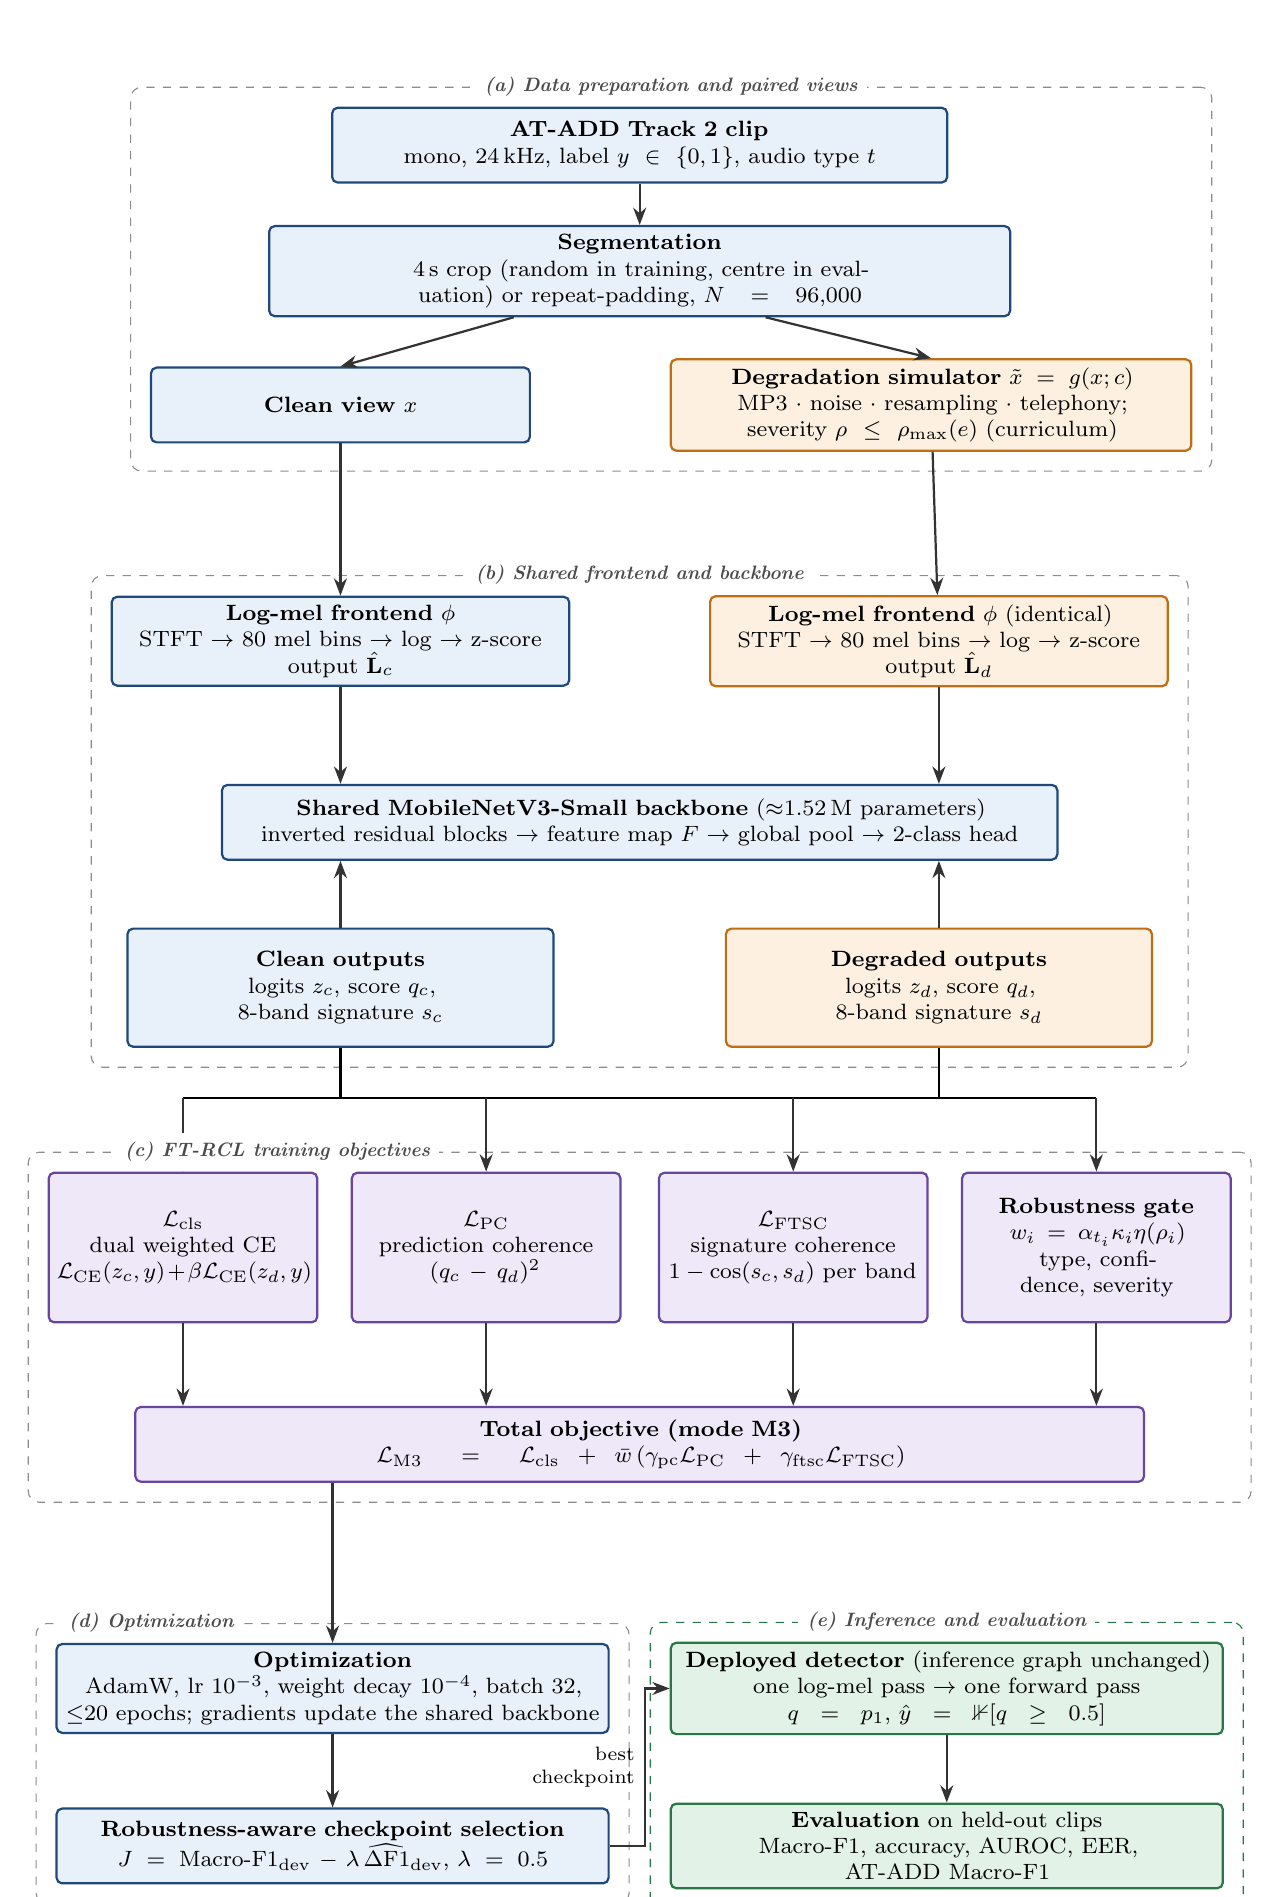
\begin{tikzpicture}
% (a) data preparation and paired views
\node[blk,text width=7.6cm] (in) at (0,0) {\textbf{AT-ADD Track~2 clip}\\mono, 24\,kHz, label $y\in\{0,1\}$, audio type $t$};
\node[blk,text width=9.2cm] (seg) at (0,-1.6) {\textbf{Segmentation}\\4\,s crop (random in training, centre in evaluation) or repeat-padding, $N=96{,}000$};
\node[blk,text width=4.6cm] (xc) at (-3.8,-3.3) {\textbf{Clean view} $x$};
\node[trn,text width=6.4cm] (g) at (3.7,-3.3) {\textbf{Degradation simulator} $\tilde{x}=g(x;c)$\\MP3 $\cdot$ noise $\cdot$ resampling $\cdot$ telephony;\\severity $\rho\le\rho_{\max}(e)$ (curriculum)};
% (b) frontend and backbone
\node[blk,text width=5.6cm] (mc) at (-3.8,-6.3) {\textbf{Log-mel frontend} $\phi$\\STFT $\to$ 80 mel bins $\to$ log $\to$ z-score\\output $\hat{\mathbf L}_c$};
\node[trn,text width=5.6cm] (md) at (3.8,-6.3) {\textbf{Log-mel frontend} $\phi$ (identical)\\STFT $\to$ 80 mel bins $\to$ log $\to$ z-score\\output $\hat{\mathbf L}_d$};
\node[blk,text width=10.4cm] (bb) at (0,-8.6) {\textbf{Shared MobileNetV3-Small backbone} ($\approx$1.52\,M parameters)\\inverted residual blocks $\to$ feature map $F$ $\to$ global pool $\to$ 2-class head};
\node[blk,text width=5.2cm,minimum height=1.5cm] (oc) at (-3.8,-10.7) {\textbf{Clean outputs}\\logits $z_c$, score $q_c$,\\8-band signature $s_c$};
\node[trn,text width=5.2cm,minimum height=1.5cm] (od) at (3.8,-10.7) {\textbf{Degraded outputs}\\logits $z_d$, score $q_d$,\\8-band signature $s_d$};
% (c) objectives
\node[los,text width=3.2cm,minimum height=1.9cm] (lcls) at (-5.8,-14.0) {$\mathcal{L}_{\mathrm{cls}}$\\dual weighted CE\\$\mathcal{L}_{\mathrm{CE}}(z_c,y)+\beta\mathcal{L}_{\mathrm{CE}}(z_d,y)$};
\node[los,text width=3.2cm,minimum height=1.9cm] (lpc) at (-1.95,-14.0) {$\mathcal{L}_{\mathrm{PC}}$\\prediction coherence\\$(q_c-q_d)^2$};
\node[los,text width=3.2cm,minimum height=1.9cm] (lft) at (1.95,-14.0) {$\mathcal{L}_{\mathrm{FTSC}}$\\signature coherence\\$1-\cos(s_c,s_d)$ per band};
\node[los,text width=3.2cm,minimum height=1.9cm] (gate) at (5.8,-14.0) {\textbf{Robustness gate}\\$w_i=\alpha_{t_i}\kappa_i\eta(\rho_i)$\\type, confidence, severity};
\node[los,text width=12.6cm] (tot) at (0,-16.5) {\textbf{Total objective (mode M3)}\\$\mathcal{L}_{\mathrm{M3}}=\mathcal{L}_{\mathrm{cls}}+\bar{w}\,(\gamma_{\mathrm{pc}}\mathcal{L}_{\mathrm{PC}}+\gamma_{\mathrm{ftsc}}\mathcal{L}_{\mathrm{FTSC}})$};
% (d) optimisation and (e) inference side by side
\node[blk,text width=6.8cm] (opt) at (-3.9,-19.6) {\textbf{Optimization}\\AdamW, lr $10^{-3}$, weight decay $10^{-4}$, batch 32, $\le$20 epochs; gradients update the shared backbone};
\node[blk,text width=6.8cm] (sel) at (-3.9,-21.6) {\textbf{Robustness-aware checkpoint selection}\\$J=\mathrm{Macro\text{-}F1}_{\mathrm{dev}}-\lambda\,\widehat{\Delta\mathrm{F1}}_{\mathrm{dev}}$, $\lambda=0.5$};
\node[dep,text width=6.8cm] (inf) at (3.9,-19.6) {\textbf{Deployed detector} (inference graph unchanged)\\one log-mel pass $\to$ one forward pass\\$q=p_1$, $\hat y=\mathbb 1[q\ge0.5]$};
\node[dep,text width=6.8cm] (ev) at (3.9,-21.6) {\textbf{Evaluation} on held-out clips\\Macro-F1, accuracy, AUROC, EER,\\AT-ADD Macro-F1};
% arrows
\draw[arr] (in)--(seg);
\draw[arr] ([xshift=-1.6cm]seg.south)--(xc.north);
\draw[arr] ([xshift=1.6cm]seg.south)--(g.north);
\draw[arr] (xc)--(mc);
\draw[arr] (g)--(md);
\draw[arr] (mc.south)--(mc.south |- bb.north);
\draw[arr] (md.south)--(md.south |- bb.north);
\draw[arr] (oc.north)--(oc.north |- bb.south);
\draw[arr] (od.north)--(od.north |- bb.south);
\draw[thick] (oc.south)--(oc.south |- 0,-12.1);
\draw[thick] (od.south)--(od.south |- 0,-12.1);
\draw[thick] (-5.8,-12.1)--(5.8,-12.1);
\foreach \n in {lcls,lpc,lft,gate}{\draw[arr] (\n.north |- 0,-12.1)--(\n.north);}
\foreach \n in {lcls,lpc,lft,gate}{\draw[arr] (\n.south)--(\n.south |- tot.north);}
\draw[arr] (tot.south -| opt.north)--(opt.north);
\draw[arr] (opt)--(sel);
\draw[arr] (sel.east)--++(0.45,0)|-node[pos=0.25,left,font=\scriptsize,align=right]{best\\checkpoint}(inf.west);
\draw[arr] (inf)--(ev);
% stage frames
\begin{scope}[on background layer]
\node[stage,fit=(in)(seg)(xc)(g)] (sA) {};
\node[stage,fit=(mc)(md)(bb)(oc)(od)] (sB) {};
\node[stage,fit=(lcls)(lpc)(lft)(gate)(tot)] (sC) {};
\node[stage,fit=(opt)(sel)] (sD) {};
\node[stage,fit=(inf)(ev),draw=deployedge] (sE) {};
\end{scope}
\node[stlab,fill=white,anchor=center] at (sA.north) {(a) Data preparation and paired views};
\node[stlab,fill=white,anchor=center] at (sB.north) {(b) Shared frontend and backbone};
\node[stlab,fill=white,anchor=center] at ([xshift=-4.6cm]sC.north) {(c) FT-RCL training objectives};
\node[stlab,fill=white,anchor=west] at ([xshift=0.3cm]sD.north west) {(d) Optimization};
\node[stlab,fill=white,anchor=center] at (sE.north) {(e) Inference and evaluation};
\end{tikzpicture}}
\caption{Overall end-to-end workflow of the proposed methodology. Orange blocks are used only during training; the deployed detector (green) keeps the single-view baseline inference graph.}
\label{fig:pipeline-overview}
\end{figure}


\section{Problem formulation}
\label{sec:formulation}

Let $x \in \mathbb{R}^{N}$ be a mono waveform with sampling rate $f_s = 24{,}000$\,Hz and fixed length $N = 4 f_s = 96{,}000$ samples (four seconds). The label $y \in \{0,1\}$ indicates real ($0$) or fake ($1$). The classifier produces logits $z \in \mathbb{R}^2$ and probabilities $p = \mathrm{softmax}(z)$. The \textbf{detection score} used for ROC analysis and EER is the fake-class probability $q = p_1$.

For robustness training, a condition $c$ from a finite catalogue defines a waveform-domain operator $g(\cdot\,; c)$. The paired sample $(x, \tilde{x})$ satisfies $\tilde{x} = g(x; c)$ with the same label $y$ and the same temporal crop. Mel extraction $\phi(\cdot)$ is applied \textbf{identically} to both waveforms:
\begin{equation}
\mathbf{X} = \phi(x), \qquad \tilde{\mathbf{X}} = \phi(\tilde{x}).
\label{eq:pair}
\end{equation}
Degradation never alters the mel hyperparameters or normalization statistics, which ensures a fair comparison with the clean baseline.

\section{Dataset and evaluation protocol}
\label{sec:data}

\subsection{AT-ADD Track 2}
\label{sec:data-track2}

AT-ADD Track 2 provides real/fake labels and audio-type annotations for speech, singing, music, and environmental sound. Generator metadata is available for fake audio samples. The present study uses project-specific manifest files prepared from the broader AT-ADD Track 2 dataset. The sample counts reported in the following sections refer to these manifests and should not be interpreted as the total size of the complete benchmark.

The three manifests define the working dataset used in this study: 60,000 training samples, 22,536 development samples, and 44,289 evaluation samples. All records listed in these manifests were used in the reported experiments. The partitioning procedure and the resulting generator and speaker separation are described in Section~\ref{sec:partitioning}, while Section~\ref{sec:data-used} specifies how the manifest-defined data were used for training, validation, and evaluation.

\subsection{Dataset Partitioning and Split Integrity}
\label{sec:partitioning}
\label{sec:overlap}

The original training and development data can share fake-audio generators, which may lead to optimistic validation results when a detector learns generator-specific characteristics. To address this issue, the project-specific data were organised into generator-disjoint training, development, and evaluation manifests. The resulting partitions were audited to examine generator overlap and speaker-ID overlap.

The three manifests contain 126,825 audio samples in total, distributed across 60,000 training samples, 22,536 development samples, and 44,289 evaluation samples. These counts describe the working dataset used in this study rather than the complete AT-ADD Track 2 collection. Table~\ref{tab:dataset-manifests} summarises the distribution of samples across the three manifests by class and audio type.

\begin{table}[htbp]
\centering
\caption{Sample distribution across the manifest-defined dataset partitions.}
\label{tab:dataset-manifests}
\label{tab:dataset-eval}
\small
\begin{tabular}{@{}lrrrrrrr@{}}
\toprule
Partition & Real & Fake & Total & Speech & Singing & Music & Sound \\
\midrule
Training    & 16{,}000 & 44{,}000 & 60{,}000  & 34{,}000 & 8{,}000 & 10{,}000 & 8{,}000 \\
Development & 6{,}536  & 16{,}000 & 22{,}536  & 12{,}000 & 4{,}000 & 2{,}536  & 4{,}000 \\
Evaluation  & 6{,}536  & 37{,}753 & 44{,}289  & 27{,}000 & 6{,}753 & 4{,}536  & 6{,}000 \\
\midrule
\textbf{Total} & \textbf{29{,}072} & \textbf{97{,}753} & \textbf{126{,}825} & \textbf{73{,}000} & \textbf{18{,}753} & \textbf{17{,}072} & \textbf{18{,}000} \\
\bottomrule
\end{tabular}
\end{table}

The manifest-defined dataset is imbalanced towards fake audio. Fake samples account for approximately 73.33\% of the training set, 71.00\% of the development set, and 85.24\% of the evaluation set. This imbalance is important when interpreting pooled evaluation metrics, particularly because the audio-type distributions also differ across partitions. Accordingly, pooled metrics are considered alongside audio-type-averaged Macro-F1 to assess performance across speech, singing, music, and sound.

\paragraph{Generator-wise partitioning.} The generator metadata was examined to determine whether fake-audio generators were shared across the three manifests. The training set contains 21 distinct generator names, the development set contains 8, and the evaluation set contains 38. No exact generator name is shared between any pair of partitions. This means that the fake-audio generator groups in the training, development, and evaluation manifests are disjoint according to the generator labels recorded in the files.

The training manifest contains 44,000 fake samples from 21 generators. AudioLDM2 contributes 4,000 samples. AudioLDM, DiffSpeech, FastDiff, FastPitch, FastSpeech2, Glow-TTS, GradTTS, Index-TTS, Kokoro, MelGAN, MusicLDM, NeuCoSVC\_inhouse, Parler-TTS (mini), PortaSpeech (normal), ProDiff, So-VITS-SVC\_inhouse, Stable Audio open, StarGANv2-VC, Tacotron2, and WaveGlow each contribute 2,000 samples.

The development manifest contains 16,000 fake samples from eight generators: Audiogen, CosyVoice, Llasa1B, MeloTTS, MusicGen, SeedVC, Tortoise-TTS, and WaveNet. Each contributes 2,000 samples.

The evaluation manifest contains 37,753 fake samples from 38 generator labels. RVC-FSD contributes 753 samples, while ACE-Step, Auffusion, BigVGAN, Both-Ears-Wide-Open, ChatTTS, CosyVoice2, CosyVoice3, DiffGANTTS, E2TTS, F5TTS, FireRedTTS2, Fish, Free-SVC, GPTSoVITS, HiFiGAN, IndexTTS1.5, IndexTTS2, KNN-SVC, Llasa3B, Llasa8B, MBMelGAN, MeanAudio, Musictango, OpenVoice2, ParallelWaveGAN, SSM-TTM, SeedVC1, So-VITS-SVC-FSD, SparkTTS, StepAudioTTS, StyleMelGAN, StyleSpeech, StyleTTS2, UniAudio2, Uniaudio2, VEVO1.5, and VITS each contribute 1,000 samples. Generator names are retained as recorded in the manifests.

\paragraph{Speaker-ID overlap audit.} Speaker metadata was also examined to identify potential overlap between the partitions. After excluding missing identifiers, represented by \texttt{-}, and the generic \texttt{single-speaker} marker, the manifests contain 1,668 distinct explicit speaker IDs in training, 590 in development, and 1,097 in evaluation. No common explicit speaker IDs were found between training and development, training and evaluation, or development and evaluation.

Speaker identifiers are not available for all samples. The \texttt{speaker\_id} field is missing for 52,000 training records, 18,536 development records, and 40,289 evaluation records. Consequently, the audit establishes non-overlap among the available explicit speaker identifiers but cannot independently establish speaker-level separation for recordings without identifiable speaker metadata. Generator disjointness and speaker-ID disjointness are therefore treated as separate properties of the dataset partitioning.

Overall, the manifest audit establishes disjoint generator labels and disjoint explicit speaker identifiers across the three partitions. These checks support evaluation of generalisation to unseen generators and speakers where the metadata permits verification. The conclusions apply to the manifest-defined working dataset and should not be extended to samples outside these manifests without a corresponding audit.

\subsection{Data Used in the Reported Experiments}
\label{sec:data-used}

The reported experiments use all records contained in the three project-specific manifests. The baseline, FT-RCL, and STAR-Edge models use the 60,000 samples in the training manifest for model fitting and the 22,536 samples in the development manifest for validation and checkpoint selection. Final evaluation is performed on all 44,289 samples in the evaluation manifest.

The training manifest contains 16,000 real and 44,000 fake samples. The development manifest contains 6,536 real and 16,000 fake samples, while the evaluation manifest contains 6,536 real and 37,753 fake samples. All four audio categories are represented in each partition. No additional sampling was performed from these manifests for the reported experiments.

The evaluation results therefore correspond to the complete evaluation manifest rather than smaller exploratory subsets. However, the 44,289 evaluated samples represent the evaluation data selected for this study and should not be described as the entirety of the broader AT-ADD Track 2 collection unless that scope is independently established.

No evaluation-manifest samples are used for parameter updates or checkpoint selection. The development set is used for validation, while the evaluation set is reserved for final performance assessment. Since the generator labels are disjoint across the manifests, the evaluation protocol measures generalisation to generator labels not present in the training or development data. The reported results should be interpreted in the context of the manifest-defined dataset size, its class imbalance, its audio-type distribution, and the limitations of the available speaker metadata.

\section{Audio preprocessing and log-mel frontend}
\label{sec:frontend}

\subsection{Loading and segmentation}

Audio clips are converted to mono and resampled to $f_s = 24\,\text{kHz}$ to match the AT-ADD Track~2 evaluation standard. Each clip is formatted to a fixed duration of $N = 4 \times f_s = 96{,}000$ samples (four seconds). A recording longer than four seconds is cropped to length $N$ using a random start offset during training (providing temporal translation augmentation) and a deterministic centre crop during evaluation. A recording shorter than four seconds ($L < N$) is extended to length $N$ by periodic tiling (repeat-padding), $x_{\mathrm{pad}}[n] = x[n \pmod L]$. As justified in Section~\ref{sec:duration-norm}, repeat-padding is adopted as a controlled preprocessing choice to avoid the deterministic trailing-silence cue introduced by zero-padding, recognizing that repetition boundaries may introduce a waveform discontinuity.

\subsection{Short-time Fourier transform and mel filtering}

With a Hann window $w[n]$, frame length $L_w = 600$ samples (25\,ms), hop $H = 240$ samples (10\,ms), and FFT size $N_{\mathrm{FFT}} = 1024$ (the window is zero-padded to the FFT size),
\begin{equation}
X(m,k) = \sum_{n=0}^{L_w-1} x[n + mH]\, w[n]\, e^{-j2\pi kn / N_{\mathrm{FFT}}}, \qquad P(m,k) = |X(m,k)|^2 .
\label{eq:stft}
\end{equation}
Frames are centred using reflection padding, so a four-second segment yields $T_m = 1 + \lfloor N/H \rfloor = 401$ frames. A mel filter bank $\mathbf{W}_{\mathrm{mel}} \in \mathbb{R}^{80 \times 513}$ with 80 bands (Slaney normalization) gives the mel power $\mathbf{P}_{\mathrm{mel}} = \mathbf{W}_{\mathrm{mel}} \mathbf{P}^{\top}$, and the log-mel features are
\begin{equation}
\mathbf{L} = \log(\mathbf{P}_{\mathrm{mel}} + \varepsilon), \qquad \varepsilon = 10^{-10}.
\label{eq:logmel}
\end{equation}

\subsection{Global normalization}

The mean $\mu$ and standard deviation $\sigma$ are computed across all time-frequency bins of the 60{,}000-sample training manifest ($\mu \approx -9.128$, $\sigma \approx 6.774$) and applied globally to training, development, and evaluation splits:
\begin{equation}
\hat{\mathbf{L}} = (\mathbf{L} - \mu) / \sigma .
\label{eq:norm}
\end{equation}
The normalized tensor $\hat{\mathbf{L}}$ is formatted as a single-channel feature representation of shape $1 \times 80 \times T_m$ for input to the convolutional backbones (Figure~\ref{fig:mel-frontend}).

\begin{figure}[htbp]
\centering
\resizebox{\linewidth}{!}{%
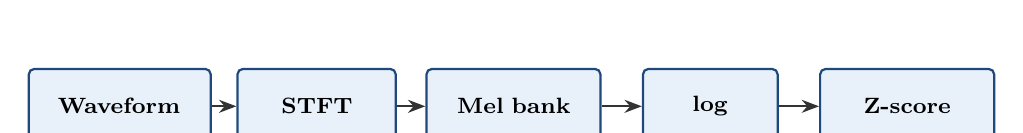
\begin{tikzpicture}
\node[blk,text width=2.1cm] (w) at (0,0) {\textbf{Waveform}};
\node[blk,text width=1.8cm] (s) at (2.5,0) {\textbf{STFT}};
\node[blk,text width=2.0cm] (m) at (5.0,0) {\textbf{Mel bank}};
\node[blk,text width=1.5cm] (l) at (7.5,0) {\textbf{log}};
\node[blk,text width=2.0cm] (z) at (10.0,0) {\textbf{Z-score}};
\draw[arr] (w)--(s);
\draw[arr] (s)--(m);
\draw[arr] (m)--(l);
\draw[arr] (l)--(z);
\end{tikzpicture}}
\caption{Audio preprocessing and log-mel feature extraction.}
\label{fig:mel-frontend}
\end{figure}


\section{Synthetic degradation (paired views)}
\label{sec:degradation}

\subsection{Degradation catalogue}

Degradations are applied to the waveform before $\phi$. Table~\ref{tab:degradations} lists the catalogue used in training. MP3 coding uses FFmpeg (libmp3lame), additive noise is white Gaussian noise scaled to a target SNR, and the telephony condition is a fourth-order Butterworth band-pass. Each degraded clip records its family, severity and random seed.

Two properties of the catalogue need to be stated. First, the resampling condition (24\,kHz $\rightarrow$ 16\,kHz $\rightarrow$ 24\,kHz) does nothing to this corpus, because the audio is natively 16\,kHz; it is an identity operation, which explains why its measured $\Delta M$ is exactly zero (Section~\ref{sec:robustness-pilot}). Second, in the implementation used for the reported runs, the noise of a deterministic degradation was drawn from the same seed for every clip, so all clips received the same noise waveform. This has been corrected: the seed now depends on the condition and the clip identifier.

\begin{table}[htbp]
\centering
\caption{Degradation families and severity levels of the training catalogue.}
\label{tab:degradations}
\small
\begin{tabular}{@{}lll@{}}
\toprule
Family & Setting & Severity $\rho$ \\
\midrule
Resample & 24\,kHz $\rightarrow$ 16\,kHz $\rightarrow$ 24\,kHz (identity on this corpus) & 1 \\
MP3 codec & 128 / 64 / 32\,kbps & 2 / 3 / 4 \\
Additive noise & SNR 20 / 10 / 5\,dB & 2 / 3 / 4 \\
Telephony & Band-pass 300--3400\,Hz & 3 \\
\bottomrule
\end{tabular}
\end{table}

The training catalogue and the evaluation conditions are the same families. A test of generalisation therefore needs conditions that were not used in training, for instance AAC, Opus, G.711 telephony, reverberation and packet loss. Such conditions are implemented in the evaluation code but their results are not available (Section~\ref{sec:robustness-pilot}).

\figimage{spectrogram-pairs}{Clean and degraded versions of one evaluation clip as waveform and log-mel spectrogram.}{figures/plots/btp_report/spectrogram_pairs.png}

\subsection{Severity levels and curriculum}

The severity $\rho$ is an ordinal rank used to schedule the curriculum and to scale the gate. It increases within a family as the bitrate or SNR falls, but the ranks of different families are a design choice and not a calibrated quantity: MP3 at 128\,kbps and noise at 20\,dB share rank~2 without being equally damaging. The agreement between assigned rank and measured drop could not be checked because the degraded-audio results are not valid.

Let $\rho_{\max}(e)$ be the largest severity allowed at epoch $e$, with milestones at epochs 6 and 13:
\begin{equation}
\rho_{\max}(e) = \begin{cases}
1 & e < 6, \\
3 & 6 \le e < 13, \\
4 & e \ge 13 .
\end{cases}
\label{eq:curriculum}
\end{equation}
Only conditions with $\rho \le \rho_{\max}(e)$ should be sampled (Figure~\ref{fig:m3-gating}). Two facts limit what this schedule meant in practice. The FT-RCL run stopped at epoch 12 by early stopping, so it never reached the $\rho=4$ stage, and its best checkpoint is from epoch 7. More importantly, the training loader used persistent worker processes, each of which keeps its own copy of the dataset; the severity cap was set in the main process and never reached the workers, so every worker sampled all severities from the first epoch. The curriculum was therefore not in effect in the reported runs. The cap is now kept in shared memory and each worker has its own random stream.

\figimage{m3-gating}{Intended severity curriculum: maximum allowed severity $\rho_{\max}$ versus epoch. In the reported runs the cap did not reach the data-loading workers.}{figures/plots/btp_report/m3_gating_curriculum.png}

The severity factor of the M3 gate (Section~\ref{sec:losses}) is
\begin{equation}
\eta(\rho) = \min\!\left(1,\ \frac{\rho}{\rho_{\max}(e)}\right).
\label{eq:eta}
\end{equation}

\section{Clean baseline model selection (mode M0)}
\label{sec:baseline}

Three candidate detector configurations were evaluated during the clean baseline stage before selecting the model to be carried forward into subsequent experiments, representing a structured representation progression:
\begin{itemize}
  \item \textbf{E1 (Compact CNN reference):} used a scratch-trained MobileNetV3-Small~\cite{howard2019mobilenetv3} operating on the compact 80-bin log-mel representation, with depthwise-separable convolutions and inverted bottlenecks ($1{,}519{,}618$ parameters), drawing architectural motivation from lightweight vision-backbone studies in audio deepfake detection~\cite{pham2024deepfake}.
  \item \textbf{E2 (Temporal baseline):} extended the MobileNetV3-Small convolutional representation with a one-layer GRU with hidden size 128 ($1{,}198{,}082$ parameters) to investigate whether explicit temporal sequence modelling improved the compact detector over global spatial pooling, following convolutional-recurrent designs evaluated in literature~\cite{pham2024deepfake}.
  \item \textbf{E3 (Strong learned representation):} adapted PANNs MobileNetV2~\cite{kong2020panns} initialized with AudioSet-pretrained weights and a newly initialized binary real/fake classification head ($3{,}537{,}250$ parameters). Motivated by evidence that pretrained audio representations transfer rich discriminative priors~\cite{combei2024wavlm,kong2020panns}, this experiment investigated whether general-purpose audio pretraining provided a stronger starting point for deepfake detection than learning the representation entirely from scratch.
\end{itemize}

All three configurations were evaluated using three independent training seeds (seeds 42, 1337, and 2024) under the standardized baseline protocol with gradient clipping ($\text{MAX\_GRAD\_NORM}=5.0$). E3 achieved the strongest clean performance across all metrics (type-averaged Macro-F1 of $0.6274 \pm 0.0158$, AUROC of $0.8800 \pm 0.0032$, and EER of $0.1993 \pm 0.0028$) and demonstrated substantially lower variation across seeds. It was therefore selected as the clean reference baseline \textbf{M0}. From this point onward, \textbf{M0 refers specifically to E3} (Figure~\ref{fig:mobilenet-baseline}).

\begin{figure}[htbp]
\centering
\resizebox{\linewidth}{!}{%
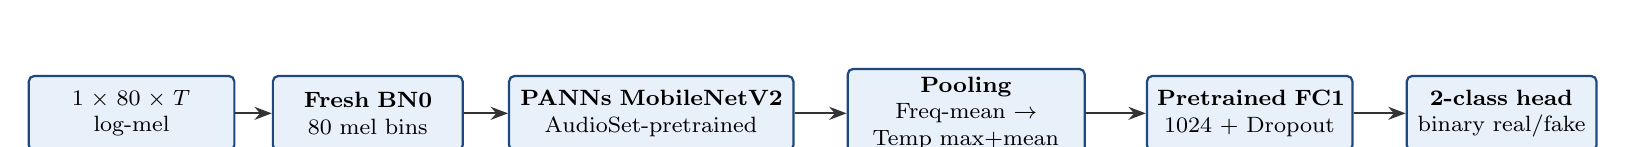
\begin{tikzpicture}
\node[blk,text width=2.4cm] (in) at (0,0) {$1\times80\times T$\\log-mel};
\node[blk,text width=2.2cm] (bn) at (3.0,0) {\textbf{Fresh BN0}\\$80$ mel bins};
\node[blk,text width=3.4cm] (mn) at (6.6,0) {\textbf{PANNs MobileNetV2}\\AudioSet-pretrained};
\node[blk,text width=2.8cm] (gp) at (10.6,0) {\textbf{Pooling}\\Freq-mean $\to$ Temp max+mean};
\node[blk,text width=2.4cm] (fc) at (14.2,0) {\textbf{Pretrained FC1}\\$1024$ + Dropout};
\node[blk,text width=2.2cm] (hd) at (17.4,0) {\textbf{2-class head}\\binary real/fake};
\draw[arr] (in)--(bn);
\draw[arr] (bn)--(mn);
\draw[arr] (mn)--(gp);
\draw[arr] (gp)--(fc);
\draw[arr] (fc)--(hd);
\end{tikzpicture}}
\caption{Selected clean baseline architecture M0 (PANNs MobileNetV2 with AudioSet-pretrained feature extractor, fresh 80-bin BN0, and binary classification head; $3{,}537{,}250$ parameters).}
\label{fig:mobilenet-baseline}
\label{fig:panns-baseline}
\end{figure}


\subsection{Class-weighted cross-entropy loss}

With class counts $n_0, n_1$ and total $n = n_0 + n_1$, the weights $\omega_j = n / (2 n_j)$ balance the real and fake classes:
\begin{equation}
\mathcal{L}_{\mathrm{CE}}(z, y) = -\sum_{j \in \{0,1\}} \omega_j \,\mathbb{1}[y=j]\,\log p_j .
\label{eq:ce}
\end{equation}
For the $16{,}000:44{,}000$ (real:fake) ratio of the training manifest ($n=60{,}000$), this gives $\omega_0 = 1.875$ for genuine audio and $\omega_1 \approx 0.682$ for synthetic audio. Mode \textbf{M0} (clean-only training with selected model E3) minimizes $\mathcal{L}_{\mathrm{CE}}$ on clean batches only.

\section{FT-RCL detector}
\label{sec:ftrcl}

\subsection{Architecture and subband signatures}

The FT-RCL detector shares the MobileNetV3 backbone and also returns the last feature map $F \in \mathbb{R}^{B \times C \times H \times W}$ with $C=576$ (Figure~\ref{fig:ft-rcl-paired}). The signature module splits the frequency axis into $K=8$ bands. For band $k$ with rows $[h_k, h_{k+1})$,
\begin{equation}
b_k = \mathrm{mean}_{h,w}\big(F_{:,:,h_k:h_{k+1},:}\big) \in \mathbb{R}^{B \times C}.
\label{eq:subband}
\end{equation}
The bands are stacked into $s^{(0)} \in \mathbb{R}^{B \times K \times C}$ and normalised along the channel axis:
\begin{equation}
s = \mathrm{normalize}\big(s^{(0)},\ p=2,\ \mathrm{dim}=-1\big).
\label{eq:signature}
\end{equation}

The question of how eight bands arise from a feature map with few rows has a direct answer: they do not. The backbone reduces frequency resolution by a factor of 32, so an input with 80 mel bins gives $H=3$ rows at the last layer. The implementation used for the reported runs assigned one row to each of the first three bands and left bands four to eight empty. The mean of an empty slice is undefined, so five of the eight signature bands were not-a-number, the logged FTSC and total loss were not-a-number in every epoch (the loss columns of the saved training logs are empty), and the training loss could not be used for monitoring. The gradients were nevertheless finite, because the undefined bands are not connected to the feature map, so training went on and the FTSC term constrained only the first three bands (one row each). We reproduced this behaviour: with the old module the loss is undefined while all parameter gradients are finite. An exploratory conjecture that the loss was unstable under mixed precision was unfounded; the exploratory runs used a CPU and no mixed precision (Chapter~\ref{ch:setup}).

The corrected module averages over time and then divides the $H$ rows into $K$ possibly overlapping bins with the boundaries used by adaptive average pooling, so that no band is empty. With $H=3$ the eight bands are still an interpolated view of three rows and not eight independent frequency bands. Taking the feature map from an earlier stage with finer frequency resolution would be a better design and is left for future work. The results of Chapter~\ref{ch:results} come from the old module, so they describe FTSC on three bands.

\begin{figure}[htbp]
\centering
\resizebox{0.92\linewidth}{!}{%
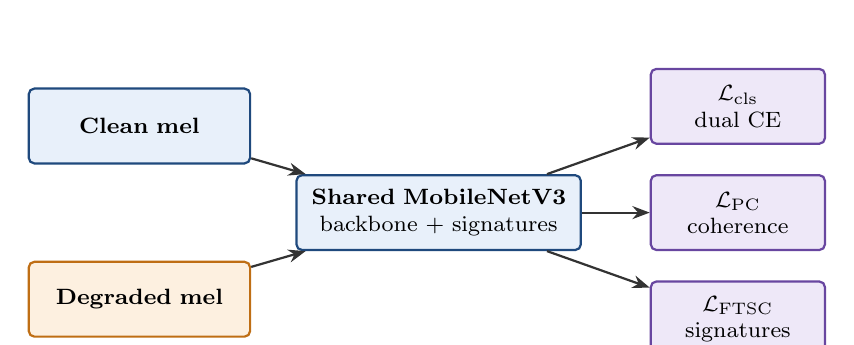
\begin{tikzpicture}
\node[blk,text width=2.6cm] (c) at (-2.2,1.1) {\textbf{Clean mel}};
\node[trn,text width=2.6cm] (d) at (-2.2,-1.1) {\textbf{Degraded mel}};
\node[blk,text width=3.4cm] (bb) at (1.6,0) {\textbf{Shared MobileNetV3}\\backbone + signatures};
\node[los,text width=2.0cm] (lcls) at (5.4,1.35) {$\mathcal{L}_{\mathrm{cls}}$\\dual CE};
\node[los,text width=2.0cm] (lpc) at (5.4,0) {$\mathcal{L}_{\mathrm{PC}}$\\coherence};
\node[los,text width=2.0cm] (lft) at (5.4,-1.35) {$\mathcal{L}_{\mathrm{FTSC}}$\\signatures};
\draw[arr] (c)--(bb);
\draw[arr] (d)--(bb);
\draw[arr] (bb)--(lcls);
\draw[arr] (bb)--(lpc);
\draw[arr] (bb)--(lft);
\end{tikzpicture}}
\caption{FT-RCL paired clean/degraded-view training architecture.}
\label{fig:ft-rcl-paired}
\end{figure}


\subsection{Loss functions}
\label{sec:losses}

Let $z_c, z_d$ be the logits from the clean and degraded mel inputs, $q_c, q_d$ the corresponding fake-class probabilities, and $s_c, s_d$ the signatures.

\subsubsection{Dual classification}

With the class-weighted cross-entropy of Equation~\eqref{eq:ce},
\begin{equation}
\mathcal{L}_{\mathrm{cls}} = \mathcal{L}_{\mathrm{CE}}(z_c, y) + \beta\,\mathcal{L}_{\mathrm{CE}}(z_d, y), \qquad \beta = 0.5 .
\label{eq:cls}
\end{equation}

\subsubsection{Prediction coherence (PC)}

\begin{equation}
\mathcal{L}_{\mathrm{PC}} = \frac{1}{B}\sum_{i=1}^{B} \big(q_{c,i} - q_{d,i}\big)^2 .
\label{eq:pc}
\end{equation}
If, for one clip, $q_c=0.80$ and $q_d=0.55$, the clip adds $0.0625$ to the sum and pushes the degraded prediction toward the clean one. PC cannot tell right from wrong, since two views can agree on the wrong label. A squared difference of probabilities also has a weak gradient when one of the two outputs is saturated near 0 or 1, which is exactly the case of a confident clean prediction and a collapsed degraded one. A Kullback--Leibler or Jensen--Shannon term on the output distributions does not have this property~\cite{hendrycks2020augmix}; we did not compare them.

\subsubsection{Feature signature coherence (FTSC)}

For band $k$ and sample $i$, let $s_{c,i,k}, s_{d,i,k} \in \mathbb{R}^{C}$ be the L2-normalized band vectors and $\cos_{i,k} = s_{c,i,k}^\top s_{d,i,k}$. FTSC compares the clean and degraded signatures by the cosine similarity along the channel dimension for each band and averages over bands and batch:
\begin{equation}
\mathcal{L}_{\mathrm{FTSC}} = \frac{1}{B}\sum_{i=1}^{B} \frac{1}{K}\sum_{k=1}^{K} (1 - \cos_{i,k}).
\label{eq:ftsc}
\end{equation}
Figure~\ref{fig:pc-ftsc} illustrates PC and FTSC.

\figimage{pc-ftsc}{Prediction coherence and feature signature coherence.}{figures/plots/btp_report/pc_ftsc.png}

\subsubsection{Type, confidence, and severity robustness gate}

For sample $i$ with audio type $t_i$, the gate combines a type weight $\alpha_{t_i}$ (defaults: speech and singing $1.0$, music $0.3$, sound $0.5$), a confidence $\kappa_i = 2|q_{c,i} - 0.5|$ (treated as a constant, so no gradient flows through $\kappa$), and the severity factor $\eta(\rho_i)$ of Equation~\eqref{eq:eta}:
\begin{equation}
w_i = \alpha_{t_i}\,\kappa_i\,\eta(\rho_i), \qquad \bar{w} = \frac{1}{B}\sum_{i=1}^{B} w_i .
\label{eq:gate}
\end{equation}
The type weights were set by hand to reduce the constraint on the two types where the baseline is weakest; they were not estimated from data and no other values were tried. The confidence term switches the coherence loss off for uncertain clean predictions, which are the samples that probably need it most. Because the batch mean $\bar w$ multiplies the batch-level coherence loss, the gate scales the loss of the whole batch and does not weight individual samples. An ungated variant would show whether the gate matters; it was not run.

\subsection{Total loss and training modes}

The total loss of the full FT-RCL objective (mode M3) is
\begin{equation}
\mathcal{L}_{\mathrm{M3}} = \mathcal{L}_{\mathrm{cls}} + \bar{w}\,\Big(\gamma_{\mathrm{pc}}\mathcal{L}_{\mathrm{PC}} + \gamma_{\mathrm{ftsc}}\mathcal{L}_{\mathrm{FTSC}}\Big), \qquad \gamma_{\mathrm{pc}} = 1.0,\ \gamma_{\mathrm{ftsc}} = 0.5 .
\label{eq:m3}
\end{equation}
Table~\ref{tab:modes} summarizes how the four training modes combine the terms of Equations~\eqref{eq:cls}--\eqref{eq:ftsc} and the gate of Equation~\eqref{eq:gate}. Mode~M1 uses $\mathcal{L}_{\mathrm{CE}}(z_d,y)$ only; mode~M2 uses $\mathcal{L}_{\mathrm{cls}} + \bar{w}\,\gamma_{\mathrm{pc}}\mathcal{L}_{\mathrm{PC}}$ with $\eta \equiv 1$ and $\gamma_{\mathrm{ftsc}} = 0$.

\begin{table}[htbp]
\centering
\caption{Training modes and their loss components.}
\label{tab:modes}
\small
\renewcommand{\arraystretch}{1.2}
\begin{tabular}{@{}llll@{}}
\toprule
Mode & Network & Views used in the loss & Loss \\
\midrule
M0 & PANNs MobileNetV2 (E3) & Clean & $\mathcal{L}_{\mathrm{CE}}(z_c,y)$ \\
M1 & FT-RCL detector & Degraded & $\mathcal{L}_{\mathrm{CE}}(z_d,y)$ \\
M2 & FT-RCL detector & Clean and degraded & $\mathcal{L}_{\mathrm{cls}} + \bar{w}\,\gamma_{\mathrm{pc}}\mathcal{L}_{\mathrm{PC}}$ ($\eta\equiv 1$) \\
M3 & FT-RCL detector & Clean and degraded & $\mathcal{L}_{\mathrm{cls}} + \bar{w}\,(\gamma_{\mathrm{pc}}\mathcal{L}_{\mathrm{PC}} + \gamma_{\mathrm{ftsc}}\mathcal{L}_{\mathrm{FTSC}})$ \\
\bottomrule
\end{tabular}
\end{table}

\section{STAR-Edge extension}
\label{sec:star-edge-method}

STAR-Edge (Severity-Trajectory and Asymmetric Robustness for Edge) adds three terms to FT-RCL. It uses the same backbone, frontend, degradation catalogue and optimisation settings.

\paragraph{Asymmetric bona-fide robustness (ABR).} Genuine recordings suffer most when compression or noise creates artefacts that look like synthesis. For the real clips of a batch ($\mathcal{R}$), ABR penalises degraded views that look more fake than the clean view by more than a margin $m=0.05$:
\begin{equation}
\mathcal{L}_{\mathrm{ABR}} = \frac{1}{|\mathcal{R}|}\sum_{i\in\mathcal{R}} \max\big(0,\ q_{d,i}-q_{c,i}+m\big).
\label{eq:abr}
\end{equation}

\paragraph{Severity trajectory coherence (STC).} STC adds the signature and probability agreement between consecutive points of a trajectory $(s^{(0)},\ldots,s^{(T)})$:
\begin{equation}
\mathcal{L}_{\mathrm{STC}} = \sum_{t=0}^{T-1}\Big[\tfrac{1}{B}\sum_i\big(1-s^{(t)\top}_i s^{(t+1)}_i\big) + \tfrac{1}{B}\sum_i\big(q^{(t)}_i-q^{(t+1)}_i\big)^2\Big].
\label{eq:stc}
\end{equation}
In the implementation the trajectory has only two points, the clean and the degraded view, so STC reduces to a second copy of the pairwise terms of FT-RCL rather than a coherence across several severities. It is applied on a random half of the training steps.

\paragraph{Channel auxiliary detection (CAD).} Four waveform statistics (RMS, crest factor, spectral flatness, zero-crossing rate) are mapped by a small MLP to an eight-dimensional channel code $u$. The pooled embedding $z$ is projected orthogonally to $u$, $z'=z-(z^\top\hat u)\hat u$ with $\hat u=u/\lVert u\rVert$, and a linear head predicts the degradation family of the degraded clip from $u$ with a cross-entropy loss. The code is detached from the projection during the first three epochs.

With weights $\rho_{\mathrm{ABR}}=0.2$ and $\delta_{\mathrm{STC}}=0.3$, the objective is $\mathcal{L}_{\mathrm{M3}}+0.2\,\mathcal{L}_{\mathrm{ABR}}+\mathcal{L}_{\mathrm{CAD}}+0.3\,\mathcal{L}_{\mathrm{STC}}$. Like the other additions, these terms are only used in training. The signature problem described above applies here as well and is worse: with CAD the signature is computed from the projected pooled embedding, which has a single row, so only one of the eight bands was defined.

\section{Optimization and checkpoint selection}
\label{sec:optimization}

\subsection{Optimiser and schedule}

Training uses AdamW~\cite{loshchilov2019adamw} with learning rate $10^{-3}$ and weight decay $10^{-4}$, batch size 32, at most 20 epochs and early stopping with patience 5 on the selection score. The learning rate follows ReduceLROnPlateau on development Macro-F1 (factor 0.5, patience 2). The runs used a CPU, so no mixed precision was involved.

\subsection{Checkpoint selection}
\label{sec:selection}

The baseline keeps the epoch with the highest development Macro-F1. FT-RCL and STAR-Edge keep the epoch with the highest robustness-aware score
\begin{equation}
J = \mathrm{MacroF1}_{\mathrm{dev,clean}} - \lambda\,\widehat{\Delta \mathrm{F1}}_{\mathrm{dev}}, \qquad \lambda = 0.5 ,
\label{eq:jscore}
\end{equation}
where $\widehat{\Delta \mathrm{F1}}_{\mathrm{dev}}$ is the drop in Macro-F1 under two quick degradations. This makes the comparison unfair in a way that cannot be separated from the method: the models are chosen by different rules. The estimate itself was also unreliable. It used the first five batches of the development list, and the list is sorted by type and label, so these 160 clips were all fake music. Macro-F1 on a single class carries no information about robustness, and the logged $\widehat{\Delta \mathrm{F1}}$ values lie between $-0.03$ and $0.04$ without a trend. In addition the estimate can be negative, in which case $J$ rewards a model for scoring better on degraded than on clean audio. The corrected implementation uses a fixed development subset stratified by type and label, all degradation families and a drop clamped at zero, and the same selection rule is available for every model.

\section{Summary of implementation corrections}
\label{sec:audit}

Reviewing the code against the results exposed the problems below. The reported results of Chapter~\ref{ch:results} come from the implementation before the corrections, except where stated; the corrections are in the code base.

\begin{enumerate}
  \item The signature module produced empty bands, so the FTSC term was defined on three bands (one for STAR-Edge) and the logged loss was undefined.
  \item The severity curriculum did not reach the persistent data-loading workers.
  \item The estimate of the robustness drop used for checkpoint selection was computed on 160 fake music clips.
  \item Deterministic degradations used one noise seed for all clips, and a missing codec tool silently returned the clean waveform instead of failing.
  \item Checkpoints were loaded in a mode that ignores missing or unexpected weights.
  \item The robustness pilot used the first rows of a sorted list (Section~\ref{sec:robustness-pilot}).
\end{enumerate}

\section{Training versus inference}
\label{sec:train-infer}

\textbf{Training (M3)} requires paired degradations, two mel computations, dual logits and signatures, and the full loss $\mathcal{L}_{\mathrm{M3}}$. \textbf{Inference} applies $\phi$ once and performs a single forward pass; signatures and degradations are omitted. This preserves the latency expected of an edge-compatible deployment (Figure~\ref{fig:train-vs-infer}).

\begin{figure}[htbp]
\centering
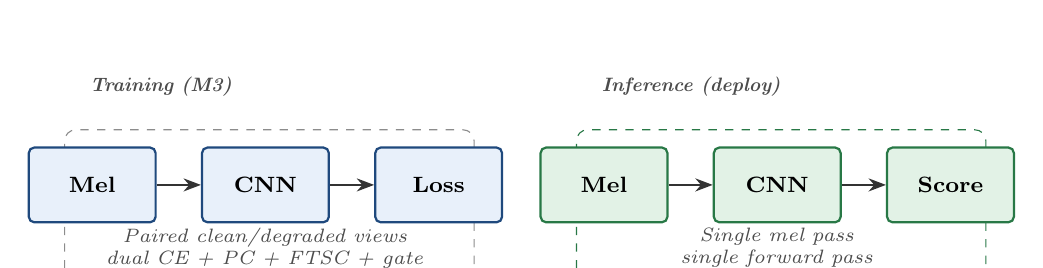
\begin{tikzpicture}
\begin{scope}
\node[font=\scriptsize\bfseries\itshape,text=black!70,anchor=south west] at (-0.15,1.35) {Training (M3)};
\draw[dashed,rounded corners=4pt,draw=black!45] (-0.35,-0.85) rectangle (4.85,1.05);
\node[blk,text width=1.4cm] (tm) at (0,0.35) {\textbf{Mel}};
\node[blk,text width=1.4cm] (tc) at (2.2,0.35) {\textbf{CNN}};
\node[blk,text width=1.4cm] (ts) at (4.4,0.35) {\textbf{Loss}};
\draw[arr] (tm)--(tc);
\draw[arr] (tc)--(ts);
\node[font=\scriptsize\itshape,text=black!70,align=center,text width=4.6cm] at (2.2,-0.45) {Paired clean/degraded views\\dual CE + PC + FTSC + gate};
\end{scope}
\begin{scope}[xshift=6.5cm]
\node[font=\scriptsize\bfseries\itshape,text=black!70,anchor=south west] at (-0.15,1.35) {Inference (deploy)};
\draw[dashed,rounded corners=4pt,draw=deployedge] (-0.35,-0.85) rectangle (4.85,1.05);
\node[dep,text width=1.4cm] (im) at (0,0.35) {\textbf{Mel}};
\node[dep,text width=1.4cm] (ic) at (2.2,0.35) {\textbf{CNN}};
\node[dep,text width=1.4cm] (is) at (4.4,0.35) {\textbf{Score}};
\draw[arr] (im)--(ic);
\draw[arr] (ic)--(is);
\node[font=\scriptsize\itshape,text=black!70,align=center,text width=4.6cm] at (2.2,-0.45) {Single mel pass\\single forward pass};
\end{scope}
\end{tikzpicture}
\caption{Training versus inference workflow.}
\label{fig:train-vs-infer}
\end{figure}


\section{Evaluation metrics}
\label{sec:evaluation-metrics}

\subsection{Metrics}

For a clip with label $y \in \{0,1\}$, the model produces logits $z$ and probabilities $p = \mathrm{softmax}(z)$ (Section~\ref{sec:formulation}). The \textbf{detection score} is
\begin{equation}
q = p_1 = \frac{e^{z_1}}{e^{z_0} + e^{z_1}} \in [0,1],
\label{eq:q}
\end{equation}
the predicted probability that the clip is fake. For a decision threshold $\tau$, the predicted label is $\hat{y}_\tau = \mathbb{1}[q \ge \tau]$. Unless stated otherwise, $\tau = 0.5$. Let $\mathrm{TP}$, $\mathrm{FP}$, $\mathrm{TN}$, and $\mathrm{FN}$ denote the counts of true positives, false positives, true negatives, and false negatives, with the fake class ($y=1$) as the positive class. The metrics are defined as follows.

\paragraph{Accuracy:} the fraction of correct decisions at threshold $0.5$ on $q$,
\begin{equation}
\mathrm{Acc} = \frac{\mathrm{TP} + \mathrm{TN}}{\mathrm{TP} + \mathrm{TN} + \mathrm{FP} + \mathrm{FN}}.
\label{eq:acc}
\end{equation}

\paragraph{Macro-F1:} the unweighted mean of the F1 scores of the real and fake classes. For class $c \in \{0,1\}$, with precision $P_c$ and recall $R_c$,
\begin{equation}
\mathrm{F1}_c = \frac{2\,P_c R_c}{P_c + R_c}, \qquad
\mathrm{Macro\text{-}F1} = \tfrac{1}{2}\left(\mathrm{F1}_0 + \mathrm{F1}_1\right),
\label{eq:macrof1}
\end{equation}
where $P_1 = \mathrm{TP}/(\mathrm{TP}+\mathrm{FP})$, $R_1 = \mathrm{TP}/(\mathrm{TP}+\mathrm{FN})$, $P_0 = \mathrm{TN}/(\mathrm{TN}+\mathrm{FN})$, and $R_0 = \mathrm{TN}/(\mathrm{TN}+\mathrm{FP})$. Unless stated otherwise, the overall values are computed over all evaluation clips pooled together.

\paragraph{AUROC:} the area under the ROC curve traced by the score $q$. With the false-positive rate $\mathrm{FPR}(\tau) = \mathrm{FP}/(\mathrm{FP}+\mathrm{TN})$ and the true-positive rate $\mathrm{TPR}(\tau) = \mathrm{TP}/(\mathrm{TP}+\mathrm{FN})$ at threshold $\tau$,
\begin{equation}
\mathrm{AUROC} = \int_{0}^{1} \mathrm{TPR}\big(\mathrm{FPR}^{-1}(u)\big)\,du
= \Pr\big(q_{+} > q_{-}\big) + \tfrac{1}{2}\Pr\big(q_{+} = q_{-}\big),
\label{eq:auroc}
\end{equation}
where $q_{+}$ and $q_{-}$ are the scores of a randomly drawn fake and real clip, respectively.

\paragraph{EER:} the error rate at the operating point where the false-positive and false-negative rates are equal. With $\mathrm{FNR}(\tau) = \mathrm{FN}/(\mathrm{FN}+\mathrm{TP})$, it is computed at the ROC point where $\mathrm{FPR}$ and $\mathrm{FNR}$ are closest,
\begin{equation}
\tau^{\ast} = \arg\min_{\tau}\,\big|\mathrm{FPR}(\tau) - \mathrm{FNR}(\tau)\big|, \qquad
\mathrm{EER} = \tfrac{1}{2}\big(\mathrm{FPR}(\tau^{\ast}) + \mathrm{FNR}(\tau^{\ast})\big).
\label{eq:eer}
\end{equation}

\paragraph{AT-ADD Macro-F1:} for each audio type $t \in \mathcal{T} = \{\text{speech}, \text{singing}, \text{music}, \text{sound}\}$, the F1 scores of the real and fake classes are averaged, and the four type-wise scores are then averaged without weighting~\cite{xie2026atadd},
\begin{equation}
\mathrm{F1}_{\mathrm{AT\text{-}ADD}} = \frac{1}{|\mathcal{T}|}\sum_{t \in \mathcal{T}} \tfrac{1}{2}\left(\mathrm{F1}_{0}^{(t)} + \mathrm{F1}_{1}^{(t)}\right),
\label{eq:atadd}
\end{equation}
where $\mathrm{F1}_{c}^{(t)}$ is the F1 score of class $c$ computed on the clips of type $t$ only. Two further quantities are reported. Because a deployed detector has one threshold for all types, the per-type results are also given at a single global threshold, taken at the pooled EER point. Calibration is summarised by the expected calibration error over 15 equal-width bins~\cite{guo2017calibration}. Intervals are 95\% percentile intervals of a clip-level bootstrap with 1000 resamples~\cite{efron1993bootstrap}; differences between models use the same resamples, so they are paired. The robustness measure is the drop $\Delta M = M_{\mathrm{clean}}-M_{\mathrm{conditioned}}$; because Macro-F1 at a fixed threshold reacts strongly to a shift in the score distribution, $\Delta$AUROC is the more reliable of the three.

No settings were tuned on evaluation data.

\chapter{Experimental Setup}
\label{ch:setup}

\section{Acoustic frontend and duration policy}
\label{sec:setup-frontend}

\subsection{AT-ADD Frontend and Duration Normalization}
\label{sec:duration-norm}

The baseline frontend follows the requirements of AT-ADD Track 2, which evaluates type-agnostic detection across speech, environmental sound, singing and music~\cite{xie2026atadd}. Audio is converted to mono, resampled to 24\,kHz, and represented using a fixed four-second input window. Longer recordings are randomly cropped during training and centre-cropped during evaluation, while shorter recordings are extended using repeat-padding.

This duration policy was motivated by the heterogeneous duration distribution of AT-ADD. The generator-level statistics used in this study show that many music and sound sources have approximately 10-second recordings, whereas numerous speech generators have median durations close to or below four seconds; for example, the median duration is 3.66\,s for ChatTTS and 3.51\,s for DiffGANTTS. Thus, a substantial portion of speech data requires extension to reach the fixed input duration. Zero-padding would introduce a deterministic trailing-silence region that is unrelated to the acoustic content and could provide a potential duration cue to the classifier. Repeat-padding avoids this particular silence pattern, although the repetition boundary may itself introduce an acoustic discontinuity.

The same frontend is used for E1, E2 and E3 so that the baseline comparison changes the detector architecture or learned representation without simultaneously changing the input preprocessing.

\section{Compute and software}
\label{sec:compute}

Experiments were implemented in PyTorch using CUDA-accelerated training with automatic mixed precision. Audio was decoded using SoundFile and resampled with librosa; MP3 coding for degradation simulations uses FFmpeg. Random seeds were fixed (seeds 42, 1337, and 2024 for the three-seed baseline experiments; seed 42 for exploratory downstream models).

\section{Training budget}
\label{sec:budget}

The clean baseline candidate models (E1, E2, E3) were trained on the 60{,}000-sample training manifest with a standardized maximum budget of 25 epochs. In all cases the model checkpoint was selected based on the highest Macro-F1 on the 22{,}536-sample development manifest. Although the training run for E1 seed~1 was permitted to run for 35 epochs, its best validation checkpoint occurred early at epoch~7 (before epoch~10); its reported metrics therefore faithfully reflect the standardized 25-epoch budget. Downstream exploratory models (FT-RCL and STAR-Edge) were trained under a 20-epoch budget on the MobileNetV3-Small backbone with early stopping (patience 5).

\section{Hyper-parameters}
\label{sec:hyper}

Table~\ref{tab:hyper} details the training configuration for the baseline selection experiments, distinguishing shared signal-processing settings from model-specific optimiser schedules. All three baseline candidates incorporate gradient clipping ($\text{MAX\_GRAD\_NORM}=5.0$) where gradients are unscaled from mixed precision prior to clipping.

\begin{table}[htbp]
\centering
\caption{Training configuration for clean baseline candidate experiments and downstream models.}
\label{tab:hyper}
\small
\begin{adjustbox}{max width=\textwidth}
\begin{tabular}{@{}ll@{}}
\toprule
Parameter & Value \\
\midrule
\multicolumn{2}{@{}l}{\textit{Common baseline settings (E1, E2, E3)}} \\
Input audio & 4\,s, 24\,kHz, 80-bin log-mel (window 600, hop 240, FFT 1024) \\
Normalisation & Training-set global z-score ($\mu \approx -9.128$, $\sigma \approx 6.774$) \\
Optimiser & AdamW, weight decay $10^{-4}$ \\
Batch size & 32 \\
Epochs budget & 25 epochs \\
Checkpoint criterion & Maximum development Macro-F1 \\
Gradient clipping & Norm clipping with $\text{MAX\_GRAD\_NORM} = 5.0$ (unscaled prior to clipping) \\
Random seeds & 3 independent seeds (42, 1337, 2024) \\
Loss function & Class-weighted cross-entropy ($\omega_0 = 1.875$, $\omega_1 \approx 0.682$) \\
\midrule
\multicolumn{2}{@{}l}{\textit{Model-specific settings}} \\
E1 (MobileNetV3-Small) & Scratch, 1{,}519{,}618 params; uniform lr $10^{-3}$; ReduceLROnPlateau (factor 0.5, patience 3) \\
E2 (MobileNetV3-Small + GRU) & Scratch, 1{,}198{,}082 params; uniform lr $10^{-3}$; ReduceLROnPlateau (factor 0.5, patience 3) \\
E3 / M0 (PANNs MobileNetV2) & AudioSet-pretrained, 3{,}537{,}250 params; frozen pretrained BN stats; \\
 & Layer-wise lr: features $10^{-5}$, FC1 $5\times 10^{-5}$, fresh BN0 $3\times 10^{-4}$, classifier $3\times 10^{-4}$; \\
 & ReduceLROnPlateau (factor 0.5, patience 3, min lr $10^{-6}$) \\
\midrule
\multicolumn{2}{@{}l}{\textit{Downstream models (exploratory MobileNetV3-Small runs)}} \\
FT-RCL (M3) & $\beta=0.5$, $\gamma_{\mathrm{pc}}=1.0$, $\gamma_{\mathrm{ftsc}}=0.5$, $K=8$; type weights $\alpha_t$ (speech/singing 1.0, sound 0.5, music 0.3); \\
 & 20 epochs, seed 42, $J$-score checkpoint selection \\
STAR-Edge (S) & ABR ($m=0.05$), STC, CAD; 20 epochs, seed 42, $J$-score checkpoint selection \\
\bottomrule
\end{tabular}
\end{adjustbox}
\end{table}

\section{Catalogue of experiments}
\label{sec:cat}

Every experiment evaluated in this study is listed in Table~\ref{tab:catalogue} with a unified identifier.

\begin{table}[htbp]
\centering
\caption{Experiments reported in this work.}
\label{tab:catalogue}
\small
\begin{adjustbox}{max width=\textwidth}
\begin{tabular}{@{}p{1.1cm}p{6.3cm}p{6.6cm}@{}}
\toprule
ID & Experiment & Purpose and Setting \\
\midrule
P4 & Re-implementation of published MobileNetV3 system~\cite{pham2024deepfake} & ASVspoof~2019 LA architectural reference \\
\midrule
E1 & MobileNetV3-Small scratch baseline & Compact CNN candidate, 3 seeds (42, 1337, 2024), 25 epochs \\
E2 & MobileNetV3-Small + 1-layer GRU & Temporal sequence candidate, 3 seeds, 25 epochs \\
E3 & PANNs MobileNetV2, AudioSet-pretrained & Pretrained audio representation candidate, 3 seeds, 25 epochs \\
M0 & Selected clean baseline (E3 configuration) & Selected clean reference model for downstream benchmarks \\
\midrule
M3 & FT-RCL (full objective) & Dual-view coherence on MobileNetV3-Small backbone, seed 42 \\
S & STAR-Edge & Extension on MobileNetV3-Small backbone, seed 42 \\
R & Degraded-audio pilot on MobileNetV3-Small and FT-RCL & Fake music clips only (not valid) \\
C & Shortcut-cue analysis & About 6{,}000 training and 6{,}000 evaluation clips \\
D & Duration and padding statistics & All 126{,}825 clips \\
\bottomrule
\end{tabular}
\end{adjustbox}
\end{table}

Modes M1 and M2 of Table~\ref{tab:modes} are defined but were not run.

\chapter{Preliminary Studies}
\label{ch:prelim}

Before the main comparison, a series of earlier experiments settled the frontend and the backbone. They used the complete official training lists and are reported here because they motivated later choices, not as part of the main evidence. Each configuration was run once.

\section{Frontend study on ASVspoof 2019 LA}
\label{sec:frontend-study}

Two frontends were compared on the ASVspoof~2019 logical-access evaluation list (71{,}237 clips; 25{,}380 training and 24{,}844 development clips). Setting P1 used 16\,kHz audio, a four-second zero-padded window, a 400-sample frame and a 160-sample hop. Setting P2 used 24\,kHz audio, repeat-padding, a 600-sample frame and a 240-sample hop. Backbone, recipe and seed were identical. The evaluation EER was 6.67\% for P1 and 12.49\% for P2 (Table~\ref{tab:asv-frontend}). In P1 the recall on attack A18 was above 98.6\%, in P2 it was 0.43\%.

The two settings differ in padding, sampling rate, frame length and hop at the same time, so the difference cannot be put down to padding alone. It is in line with the duration shortcut that has been reported for ASVspoof~2019~\cite{muller2021silver}: zero-padded clips let a classifier read the length of the speech. But the experiment does not isolate that effect, and the idea that P2 shows ``true'' discrimination is a hypothesis. ASVspoof~2019 LA is also natively 16\,kHz, so the 24\,kHz setting only up-samples the signal and cannot expose 8--12\,kHz vocoder artefacts. We did not run the single-factor experiments (padding only, sampling rate only) that would settle the question.

\begin{table}[htbp]
\centering
\caption{ASVspoof 2019 LA evaluation results of the frontend and head comparison (single runs).}
\label{tab:asv-frontend}
\small
\begin{tabular}{@{}llrrrr@{}}
\toprule
Setting & Head & Accuracy & Macro-F1 & AUROC & EER (\%) \\
\midrule
P1: 16\,kHz, zero-pad & CNN & 0.909 & 0.820 & 0.9688 & 6.67 \\
P1: 16\,kHz, zero-pad & CNN + GRU & 0.867 & 0.763 & 0.9599 & 7.55 \\
P1: 16\,kHz, zero-pad & CNN + LSTM & 0.865 & 0.761 & 0.9666 & 6.82 \\
P2: 24\,kHz, repeat-pad & CNN & 0.753 & 0.648 & 0.9324 & 12.49 \\
P2: 24\,kHz, repeat-pad & CNN + GRU & 0.692 & 0.597 & 0.9198 & 13.82 \\
P2: 24\,kHz, repeat-pad & CNN + LSTM & 0.710 & 0.612 & 0.9310 & 12.59 \\
\bottomrule
\end{tabular}
\end{table}

On ASVspoof~2019 the recurrent heads are within about one EER point of the CNN head under both settings. We chose the repeat-padded 24\,kHz frontend for the AT-ADD experiments to avoid the silence cue, knowing that the corpora are natively 16\,kHz and that the larger bandwidth brings no new information.

\section{Backbone study on AT-ADD Track 2}
\label{sec:backbone-study}

The CNN head (global average pooling) was compared with a one-layer GRU head (1.20\,M parameters)~\cite{cho2014gru} and a one-layer LSTM head (1.29\,M parameters)~\cite{hochreiter1997lstm} with hidden size 128 on the same convolutional extractor, which retains the time axis by pooling over frequency only, in the manner of earlier convolutional-recurrent spoofing detectors~\cite{gomez2019light,chintha2020crnn}. Table~\ref{tab:baseline-architecture-atadd} gives the results on the complete evaluation list. The CNN head has the lowest EER, 2.2 points below the LSTM head and 2.5 points below the GRU head, and the highest accuracy.

\begin{table}[htbp]
\centering
\caption{Head comparison on the complete AT-ADD Track~2 evaluation list (full training data, 20 epochs, single run).}
\label{tab:baseline-architecture-atadd}
\small
\begin{tabular}{@{}lccccc@{}}
\toprule
Head & Parameters & Accuracy & Macro-F1 & AUROC & EER (\%) \\
\midrule
CNN (global average pooling) & 1.52\,M & 0.757 & 0.678 & 0.8750 & 19.92 \\
CNN + GRU & 1.20\,M & 0.699 & 0.630 & 0.8425 & 22.43 \\
CNN + LSTM & 1.29\,M & 0.696 & 0.626 & 0.8622 & 22.15 \\
\bottomrule
\end{tabular}
\end{table}

The CNN's validation Macro-F1 on the official development list was 0.953, against 0.678 on evaluation, a gap discussed in Section~\ref{sec:generator-gap}. The result shows that recurrence gave no gain in these single runs; it does not show that recurrent models are worse in general, and the explanation that they overfit non-stationary audio remains a conjecture. Only a single convolutional extractor was tried, so the CNN head cannot be called optimal either. We kept it as the backbone because it is also the cheapest. A pretrained small audio network could improve the weak music and sound results but was not tried.

\section{Comparison with a published MobileNetV3 system}

Pham et al.~\cite{pham2024deepfake} report an EER of 48\% for an ImageNet-pretrained MobileNetV3 on three-channel linear-filterbank images of two-second slices of ASVspoof~2019 audio. We re-implemented their signal processing and score aggregation and trained with our own recipe (AdamW, cosine learning-rate decay, class-weighted loss, per-bin normalisation). The utterance-level EER was 16.85\% with AUROC 0.9180 (segment level: 17.01\%, 0.9162). The two implementations differ in optimiser, schedule, normalisation and recipe, so the gap to the published figure cannot be assigned to one cause. Likewise, the project baseline in setting P2 (EER 12.49\%) differs from this re-implementation in frontend, duration and sampling rate simultaneously, so the comparison does not show that one frontend is better. Table~\ref{tab:pham_comparison} lists the numbers; the published F1 values are weighted or majority-class scores and are not comparable with our unweighted Macro-F1.

\begin{table}[htbp]
\centering
\caption{Published and re-implemented MobileNetV3 systems and the project baselines on the ASVspoof 2019 LA evaluation list.}
\label{tab:pham_comparison}
\small
\resizebox{\textwidth}{!}{
\begin{tabular}{@{}llcccc@{}}
\toprule
System & Frontend & Accuracy (\%) & F1 / Macro-F1 & AUROC & EER (\%) \\
\midrule
\multicolumn{6}{@{}l}{\textit{Published~\cite{pham2024deepfake}}} \\
MobileNetV3 (C2) & linear filterbank, $64{\times}64{\times}3$ & 59.00 & 0.670* & 0.520 & 48.00 \\
ResNet-18 (C1) & linear filterbank, $64{\times}64{\times}3$ & 49.00 & 0.580* & 0.510 & 47.00 \\
ConvNeXt-Tiny (C7, 28.6\,M) & linear filterbank, $64{\times}64{\times}3$ & 88.00 & 0.900* & 0.960 & 7.50 \\
Best ensemble & STFT, CQT, LF, Gammatone & 90.00 & 0.910* & 0.994 & 3.00 \\
\midrule
\multicolumn{6}{@{}l}{\textit{Re-implementation (this work)}} \\
C2, segment level & linear filterbank, $64{\times}64{\times}3$ & 64.95 & 0.564 & 0.9162 & 17.01 \\
C2, utterance level & linear filterbank, $64{\times}64{\times}3$ & 64.60 & 0.561 & 0.9180 & 16.85 \\
\midrule
\multicolumn{6}{@{}l}{\textit{Project baselines}} \\
P2 (CNN) & 80-mel, 24\,kHz, repeat-pad & 75.32 & 0.648 & 0.9324 & 12.49 \\
P1 (CNN) & 80-mel, 16\,kHz, zero-pad & 90.90 & 0.820 & 0.9688 & 6.67 \\
\bottomrule
\end{tabular}}
\vspace{2pt}
\footnotesize *Weighted or majority-class F1 as reported by the authors; ours is unweighted Macro-F1.
\end{table}

\chapter{Results and Discussion}
\label{ch:results}

All numbers in this chapter come from the saved evaluation predictions of the three trained models (baseline M0, FT-RCL M3 and STAR-Edge) on the 13{,}287-clip evaluation subset of Section~\ref{sec:data}, which contains clips from all 38 unseen generators. No model was trained for this chapter beyond the runs described in Chapter~\ref{ch:setup}. Each model was trained once, so intervals describe the sampling of evaluation clips and not training variance.

\section{Clean evaluation}
\label{sec:clean-eval}

Table~\ref{tab:overall} gives the pooled results and the official type-averaged Macro-F1. The type-averaged score is the headline figure, because the pooled Macro-F1 is dominated by fake speech (61\% of the evaluation clips) and is higher than the type-averaged value for every model.

\begin{table}[htbp]
\centering
\caption{Clean evaluation on the 13{,}287-clip subset (95\% bootstrap intervals in brackets). The last column is the expected calibration error.}
\label{tab:overall}
\small
\setlength{\tabcolsep}{4pt}
\begin{adjustbox}{max width=\textwidth}
\begin{tabular}{@{}lccccc@{}}
\toprule
Model & Macro-F1 (pooled) & Type-averaged Macro-F1 & AUROC & EER & ECE \\
\midrule
Baseline (M0) & 0.672 [0.663, 0.681] & 0.587 [0.577, 0.598] & 0.852 [0.845, 0.860] & 0.216 [0.207, 0.224] & 0.209 \\
FT-RCL (M3) & 0.659 [0.649, 0.668] & 0.589 [0.578, 0.600] & 0.843 [0.835, 0.851] & 0.234 [0.225, 0.243] & 0.207 \\
STAR-Edge & 0.655 [0.646, 0.664] & 0.599 [0.588, 0.609] & 0.866 [0.859, 0.874] & 0.215 [0.206, 0.223] & 0.239 \\
\bottomrule
\end{tabular}
\end{adjustbox}
\end{table}

For the pairwise comparison the same bootstrap resamples were used for all models (Table~\ref{tab:paired}). FT-RCL is worse than the baseline on pooled Macro-F1, AUROC and EER, with intervals that exclude zero, and is indistinguishable from it on the type-averaged score. STAR-Edge has the same EER as the baseline, a higher AUROC and a higher type-averaged Macro-F1, and a lower pooled Macro-F1.

\begin{table}[htbp]
\centering
\caption{Paired differences from the baseline (model minus M0, 95\% bootstrap intervals). For EER a negative value is an improvement.}
\label{tab:paired}
\small
\begin{adjustbox}{max width=\textwidth}
\begin{tabular}{@{}lcccc@{}}
\toprule
Model & $\Delta$ Macro-F1 & $\Delta$ type-averaged Macro-F1 & $\Delta$ AUROC & $\Delta$ EER \\
\midrule
FT-RCL (M3) & $-0.013$ [$-0.020$, $-0.006$] & $+0.001$ [$-0.007$, $+0.011$] & $-0.009$ [$-0.016$, $-0.003$] & $+0.018$ [$+0.010$, $+0.027$] \\
STAR-Edge & $-0.017$ [$-0.024$, $-0.010$] & $+0.011$ [$+0.003$, $+0.020$] & $+0.013$ [$+0.007$, $+0.019$] & $-0.001$ [$-0.009$, $+0.008$] \\
\bottomrule
\end{tabular}
\end{adjustbox}
\end{table}

Pooled Macro-F1 is measured at the fixed threshold 0.5 and the models differ in how their scores are placed relative to it: at the pooled EER threshold the pooled Macro-F1 values are 0.689 (baseline), 0.670 (FT-RCL) and 0.690 (STAR-Edge). The ordering of the models therefore depends on the metric, which is another reason for reporting several.

The models are poorly calibrated. The expected calibration error is 0.21 for the baseline and FT-RCL and 0.24 for STAR-Edge (Figure~\ref{fig:calibration}); the reliability curves in Figure~\ref{fig:calibration} lie far from the diagonal. The fake share is 65\% in the training subset and 85\% in the evaluation subset, which shifts the best threshold, and thresholds at 0.5 are not meaningful operating points for these models.

\figimage{calibration}{Reliability curves of the three models on the evaluation subset.}{figures/plots/analysis/calibration.png}

\figimagepair{roc-eval}{ROC curves on the evaluation subset.}{%
figures/plots/E1_v4_btp_p30/roc_eval.png}{Baseline (AUROC 0.852)}{%
figures/plots/E7_ft_rcl_btp_p30/roc_eval.png}{FT-RCL (AUROC 0.843)}

\section{Results per audio type}
\label{sec:per-type}

Table~\ref{tab:type} gives the results per audio type, both with each type's own EER threshold and at the single pooled threshold that a type-agnostic deployment would use (Figure~\ref{fig:per-type}). Speech and singing work reasonably: the EER is between 16\% and 21\%, which is a high error rate for a detector and not what we would call usable. Music and sound are close to chance. The baseline's music AUROC is 0.63 and FT-RCL's is 0.55; EERs on these two types range from 0.34 to 0.47.

\begin{table}[htbp]
\centering
\caption{Results per audio type. Columns marked ``own'' use the EER threshold of the type, ``global'' columns use the pooled EER threshold. FPR and FNR are at the global threshold.}
\label{tab:type}
\small
\setlength{\tabcolsep}{3.5pt}
\begin{adjustbox}{max width=\textwidth}
\begin{tabular}{@{}llccccccc@{}}
\toprule
Type & Model & AUROC & EER (own) & Macro-F1 (0.5) & Macro-F1 (global) & FPR & FNR \\
\midrule
\multirow{3}{*}{Speech}  & Baseline & 0.909 & 0.162 & 0.695 & 0.717 & 0.282 & 0.095 \\
 & FT-RCL & 0.905 & 0.179 & 0.665 & 0.682 & 0.254 & 0.129 \\
 & STAR-Edge & 0.911 & 0.164 & 0.639 & 0.683 & 0.230 & 0.134 \\
\midrule
\multirow{3}{*}{Singing} & Baseline & 0.921 & 0.157 & 0.794 & 0.818 & 0.147 & 0.170 \\
 & FT-RCL & 0.874 & 0.208 & 0.764 & 0.769 & 0.206 & 0.210 \\
 & STAR-Edge & 0.884 & 0.198 & 0.748 & 0.781 & 0.196 & 0.199 \\
\midrule
\multirow{3}{*}{Music}   & Baseline & 0.634 & 0.399 & 0.393 & 0.424 & 0.188 & 0.575 \\
 & FT-RCL & 0.546 & 0.467 & 0.403 & 0.418 & 0.275 & 0.561 \\
 & STAR-Edge & 0.669 & 0.383 & 0.449 & 0.489 & 0.250 & 0.455 \\
\midrule
\multirow{3}{*}{Sound}   & Baseline & 0.633 & 0.426 & 0.467 & 0.484 & 0.229 & 0.656 \\
 & FT-RCL & 0.683 & 0.394 & 0.522 & 0.534 & 0.233 & 0.579 \\
 & STAR-Edge & 0.728 & 0.341 & 0.558 & 0.598 & 0.209 & 0.493 \\
\bottomrule
\end{tabular}
\end{adjustbox}
\end{table}

\figimage{per-type}{EER with a per-type threshold (left) and Macro-F1 with one global threshold (right), by audio type.}{figures/plots/analysis/per_type.png}

FT-RCL helps on sound and, at fixed threshold, on music, and loses on speech and singing, which is why its type-averaged score ties with the baseline. STAR-Edge is better than the baseline on music and sound and slightly worse on singing, and has the best type-averaged score. At the global threshold, the false-negative rate on music and sound is between 45\% and 66\% for every model, i.e.\ a large share of the fake music and sound clips is accepted as real. On the evaluation subset, the music class has only 160 real clips, so music results rest on very few genuine examples.

\section{Generalisation to unseen generators}
\label{sec:generators}

The 38 evaluation generators differ widely in difficulty (Figure~\ref{fig:generators}). At the pooled EER threshold the mean fake recall per generator is 0.78 for the baseline and STAR-Edge and 0.76 for FT-RCL; the number of generators with recall below 0.5 is six, five and four for baseline, FT-RCL and STAR-Edge. Speech generators such as CosyVoice~2, DiffGANTTS and VITS are detected almost perfectly. The hardest are music and sound systems: SSM-TTM is not detected at all by the baseline (recall 0.00), Auffusion reaches 0.12, MeanAudio 0.23 and ACE-Step 0.28. The speech vocoder BigVGAN is also hard (0.43 for the baseline, 0.31 for FT-RCL). A detector trained on 29 generators therefore does not extend to recent text-to-music and sound generators, which fits the weak music and sound results above.

\figimage{generators}{Fake recall per unseen generator at the pooled EER threshold, sorted by baseline recall.}{figures/plots/analysis/generators.png}

\section{Development versus evaluation scores}
\label{sec:generator-gap}

All three models score 0.91--0.93 Macro-F1 on the official development list, against 0.66--0.67 on evaluation (Figure~\ref{fig:dev-eval}). Overfitting to the development set is not the explanation, as the development set was only used to select an epoch. The cause is the composition of the splits (Section~\ref{sec:overlap}): the development list contains exactly the 29 fake generators of the training list, so its Macro-F1 measures in-generator performance, while the 38 evaluation generators are all unseen. The same gap exists for the full-data baseline (development 0.953, evaluation 0.678). A development set with held-out generators is needed for honest model selection; it can be built from the training list by removing a few generators, and would also make the comparison of checkpoint rules meaningful. We did not rerun the experiments with such a split.

\figimage{dev-eval}{Macro-F1 on the official development split (generators shared with training) and on the evaluation subset (unseen generators).}{figures/plots/analysis/dev_vs_eval.png}

\section{Training behaviour}
\label{sec:training}

Figure~\ref{fig:curves} shows the validation curves. The baseline reached its best validation score at epoch 20, the last one allowed, with a training accuracy of 0.98; its development score may still have been rising and we cannot say what it would have reached with a longer schedule. FT-RCL peaked at epoch 7 and stopped at epoch 12 by early stopping, and STAR-Edge used all 20 epochs. Because the models were trained for different numbers of effective epochs and chosen by different rules (Section~\ref{sec:selection}), part of the differences in Table~\ref{tab:overall} may come from the protocol and not from the objectives. The training-loss column of FT-RCL and STAR-Edge is empty in the saved logs for the reason given in Section~\ref{sec:ftrcl}, so the loss curves of these two models cannot be shown.

\figimage{curves}{Validation Macro-F1 and EER and training accuracy per epoch (official development split).}{figures/plots/analysis/curves.png}

\section{Shortcut cues in AT-ADD}
\label{sec:shortcuts}

We tested whether simple cues alone predict the label. For about 6{,}000 training and 6{,}000 evaluation clips (stratified by type and label) we computed the native sampling rate, the duration, loudness (RMS and peak level), the amount of silence and the bandwidth (95\% spectral roll-off and high-frequency energy ratio). A gradient-boosting classifier was fitted on each cue group on the training clips and applied to the evaluation clips.

All 5{,}786 sampled evaluation clips, real or fake, have a native sampling rate of 16\,kHz, so the sampling rate carries no information and, as far as we inspected, the corpus has no content above 8\,kHz. Loudness, silence and bandwidth cues give an AUROC between 0.49 and 0.60 on the evaluation clips in Table~\ref{tab:shortcuts}, which is close to chance (Table~\ref{tab:shortcuts}). Duration is different: it predicts the label with an AUROC well \emph{below} 0.5 (0.36 over all types, 0.33 for music and 0.32 for sound), which means that the relation between duration and label learnt on the training list is reversed on the evaluation list. In training the fake sound clips are shorter than the real ones (mean 8.3\,s against 9.9\,s), whereas in evaluation the fake music clips are longer than the real ones (mean 11.3\,s against 10.0\,s). A classifier that learnt ``shorter means fake'' on the training list is therefore wrong on the evaluation list. The cues do not show a shortcut that explains the good development scores; they do show that duration differs between real and fake clips in a way that is not stable across splits, which is a risk for models that see more than four seconds.

\begin{table}[htbp]
\centering
\caption{AUROC on the evaluation clips of classifiers that see only one group of cues (trained on the training clips). Values below 0.5 mean that the cue works in the opposite direction on the evaluation list.}
\label{tab:shortcuts}
\small
\begin{adjustbox}{max width=\textwidth}
\begin{tabular}{@{}lcccc@{}}
\toprule
Cue group & All types & Speech & Music & Sound \\
\midrule
Native sampling rate & 0.500 & 0.500 & 0.500 & 0.500 \\
Duration & 0.362 & 0.539 & 0.331 & 0.323 \\
Loudness & 0.543 & 0.596 & 0.566 & 0.494 \\
Silence & 0.523 & 0.557 & 0.585 & 0.502 \\
Bandwidth & 0.512 & 0.519 & 0.517 & 0.519 \\
All cues together & 0.456 & 0.657 & 0.299 & 0.351 \\
\bottomrule
\end{tabular}
\end{adjustbox}
\end{table}

\figimage{shortcuts}{AUROC of cue-only classifiers on the evaluation clips (all types and music).}{figures/plots/analysis/shortcuts.png}

Padding is a separate matter. Table~\ref{tab:durations} shows that about 40\% of the speech clips are shorter than four seconds and receive repeat-padding, while music and sound clips are almost all ten seconds long. The padding fraction is similar for real and fake speech, so it is not a label cue in AT-ADD, but the repeat-padded junction can be audible and we did not test its effect on detection.

\begin{table}[htbp]
\centering
\caption{Clip durations in the official training and evaluation lists: median in seconds and fraction of clips shorter than four seconds (which are repeat-padded).}
\label{tab:durations}
\small
\begin{adjustbox}{max width=\textwidth}
\begin{tabular}{@{}llrrrr@{}}
\toprule
 & & \multicolumn{2}{c}{Training} & \multicolumn{2}{c}{Evaluation} \\
\cmidrule(lr){3-4}\cmidrule(lr){5-6}
Type & Label & Median & $<$4\,s & Median & $<$4\,s \\
\midrule
Speech & real / fake & 5.1 / 4.5 & 0.32 / 0.41 & 4.6 / 4.6 & 0.40 / 0.41 \\
Singing & real / fake & 5.1 / 5.2 & 0.23 / 0.23 & 4.7 / 5.3 & 0.29 / 0.24 \\
Music & real / fake & 10.0 / 10.0 & 0.00 / 0.00 & 10.0 / 10.0 & 0.00 / 0.00 \\
Sound & real / fake & 10.0 / 10.0 & 0.00 / 0.00 & 10.0 / 10.0 & 0.06 / 0.01 \\
\bottomrule
\end{tabular}
\end{adjustbox}
\end{table}

\section{Degraded-audio pilot}
\label{sec:robustness-pilot}

The earlier version of this report included a conditioned evaluation on 100 clips per model, with the drop in Macro-F1 under resampling, noise and telephony (Table~\ref{tab:delta-m-summary}). On inspection the test is not valid and no conclusion about robustness can be drawn from it, for the following reasons.

\begin{itemize}
  \item \textbf{The clips are all fake music.} The evaluation code takes the first rows of the evaluation list, and that list is sorted by type and label. The saved output of the pilot contains only the audio type music, and Macro-F1 of a single-class sample is not defined in a useful way.
  \item \textbf{The zero for resampling is expected.} Every inspected clip is natively 16\,kHz, so the 16\,kHz round trip changes nothing.
  \item \textbf{The negative drops are an artefact.} A negative $\Delta$Macro-F1 of about $-0.3$ under noise means that the degraded audio was scored better than the clean audio. All clips were given the same noise waveform (Section~\ref{sec:degradation}), which shifts the scores of every clip in one direction; at a fixed threshold of 0.5 and with only fake examples, such a shift raises the fraction of clips called fake and hence the Macro-F1. This is a calibration effect and not robustness.
  \item \textbf{No MP3 conditions.} The codec tool was not available, and the code silently returned the clean waveform for those conditions in place of failing.
\end{itemize}

\begin{table}[htbp]
\centering
\caption{Degraded-audio pilot of the earlier version: mean $\Delta$Macro-F1 (clean minus conditioned) on 100 fake music clips. Shown for completeness; the values are not valid evidence (Section~\ref{sec:robustness-pilot}).}
\label{tab:delta-m-summary}
\small
\begin{tabular}{@{}llrr@{}}
\toprule
Condition & Severity & Baseline M0 & FT-RCL M3 \\
\midrule
Band-limit 300--3400\,Hz & 3 & 0.115 & 0.134 \\
Resample via 16\,kHz & 1 & 0.000 & 0.000 \\
Noise, SNR 20\,dB & 2 & $-0.310$ & $-0.223$ \\
Noise, SNR 10\,dB & 3 & $-0.320$ & $-0.262$ \\
Noise, SNR 5\,dB & 4 & $-0.320$ & $-0.268$ \\
\bottomrule
\end{tabular}
\end{table}


The telephony result, in which FT-RCL loses more than the baseline (0.134 against 0.115), is subject to the same objection and should not be read as evidence for or against the method. A valid test needs a type- and label-stratified sample of the whole evaluation list, per-clip noise, AUROC-based drops, the MP3 condition and conditions that were not used in training (AAC, Opus, G.711 telephony, reverberation, packet loss). The evaluation code for this was written, but the degraded-audio results are not available, so hypotheses H1, H2 and H4 remain untested.

\section{STAR-Edge}
\label{sec:star-edge}

The STAR-Edge model was trained for the full 20 epochs and evaluated like the other two models; its results are in Tables~\ref{tab:overall}--\ref{tab:type}. Relative to the baseline it gives the best AUROC (+0.013, interval excludes zero), the best type-averaged Macro-F1 (+0.011) and the best sound and music results, at an unchanged EER and a lower pooled Macro-F1. The improvement on music and sound is the largest effect in this study. Since the signature terms in STAR-Edge were defined on one band only, and it has additional ABR and CAD terms and a different stopping point from FT-RCL, we cannot attribute the gain to any one component. Without the M1 and M2 ablations and without repeated seeds the effect should be treated as a lead to follow up and not as an established result.

\figimagepair{star-edge-train-dev}{Training progress of STAR-Edge.}{%
figures/plots/E7_star_edge_btp_p30/dev_macro_f1_auroc.png}{Development Macro-F1 and AUROC}{%
figures/plots/E7_star_edge_btp_p30/training_loss_accuracy.png}{Training accuracy}

\section{Model size and cost}
\label{sec:efficiency}

The baseline and the FT-RCL detector have the same 1{,}519{,}618 parameters, and a forward pass for one four-second clip takes 36.7 million multiply-accumulate operations, counted with a profiler on the 80$\times$401 input (the FT-RCL detector adds only a pooling operation to this count). The saved checkpoints are 17.6\,MB, but this is not the deployment size: they also contain the optimiser state. The weights alone take 6.2\,MB in 32-bit floating point. Table~\ref{tab:efficiency} summarises these figures.

\begin{table}[htbp]
\centering
\caption{Cost of the network. Latency, peak memory and quantised accuracy were not measured.}
\label{tab:efficiency}
\small
\begin{adjustbox}{max width=\textwidth}
\begin{tabular}{@{}lrrrr@{}}
\toprule
Model & Parameters & MACs per clip & Weights (FP32) & Saved checkpoint \\
\midrule
Baseline (M0) & 1{,}519{,}618 & 36.7\,M & 6.2\,MB & 17.6\,MB \\
FT-RCL (M3) & 1{,}519{,}618 & 36.7\,M & 6.2\,MB & 17.6\,MB \\
\bottomrule
\end{tabular}
\end{adjustbox}
\end{table}

Whether this satisfies an edge budget cannot be said without measuring batch-one latency including the STFT and mel step, peak memory, INT8 accuracy and, ideally, a run on a phone or single-board computer. We also have no comparison with other ways of reaching a small budget, such as a distilled or pruned larger model or a small task-specific network like AASIST-L (about 85\,k parameters~\cite{jung2022aasist}), so ``lightweight'' is judged here only against the 300\,M-parameter systems of the leaderboard.

\section{Discussion}
\label{sec:discussion}

\paragraph{Why FT-RCL did not help.} The result is negative and we have no experiment that isolates the reason. Several explanations are consistent with the evidence. The signature loss acted on three bands, one row each, so FTSC was a weak constraint; the curriculum never operated, so there was no gradual introduction of hard degradations; the pairs were trained and chosen with a selection score computed on fake music, which makes checkpoint choice close to random among epochs 7--12; and the prediction coherence term has a weak gradient when one view is saturated. Moreover, FT-RCL differs from the baseline only through degradation-related terms while the evaluation measures clean generalisation to unseen generators, which these terms do not target. In that sense the clean evaluation is not a fair test of the idea, and the degraded-audio evaluation that would be one is missing.

\paragraph{Hypotheses.} Table~\ref{tab:hypotheses} summarises what the evidence says about the hypotheses of Chapter~\ref{ch:introduction}.

\begin{table}[htbp]
\centering
\caption{Status of the hypotheses.}
\label{tab:hypotheses}
\small
\begin{adjustbox}{max width=\textwidth}
\begin{tabular}{@{}lp{3.6cm}p{8cm}@{}}
\toprule
 & Status & Evidence \\
\midrule
H1 & Not tested & The degraded-audio pilot is invalid (Section~\ref{sec:robustness-pilot}). \\
H2 & Not tested & Modes M1 and M2 were not run. \\
H3 & Not met & FT-RCL EER is 1.8 points above the baseline (interval 1.0--2.7); STAR-Edge is level with the baseline. \\
H4 & Not tested & No valid degraded-audio results; unseen conditions not evaluated. \\
\bottomrule
\end{tabular}
\end{adjustbox}
\end{table}

\paragraph{What the study supports.} Compact CNN detectors reach an EER of about 16--21\% on speech and singing from unseen generators and are close to chance on music and sound. Development scores from the official split overstate this performance by a wide margin. Under these conditions a small difference between training objectives is within what a single run can resolve for most metrics, with the exception of the AUROC advantage of STAR-Edge and the clean-EER disadvantage of FT-RCL.

\chapter{Conclusion and Future Work}
\label{ch:conclusion}

\section{Conclusion}

We studied a 1.52\,M-parameter MobileNetV3-Small detector on AT-ADD Track~2 and compared a clean-trained baseline with two training-time robustness methods, FT-RCL and its extension STAR-Edge. The question was whether agreement between clean and degraded views makes a compact detector more robust without enlarging it. On the evidence we have, the answer is open.

What the data show is this. On 13{,}287 evaluation clips from 38 generators unseen in training, the baseline has a type-averaged Macro-F1 of 0.587, FT-RCL 0.589 and STAR-Edge 0.599. FT-RCL is not better than the baseline on any clean metric: its pooled Macro-F1 is 0.013 lower and its EER 1.8 points higher. STAR-Edge has the best AUROC and type-averaged score, mainly through better results on music and sound, but its pooled Macro-F1 is lower than the baseline's. All models detect speech and singing with an EER of 16--21\% and are close to chance on music and sound (EER 0.34--0.47). The 0.91--0.93 Macro-F1 on the official development split is not a sign of overfitting but of a benchmark whose development fakes come from the same 29 generators as the training fakes.

What the data do not show is whether any of the methods improves robustness to compression or noise. The degraded-audio pilot of the earlier version contained only fake music, used one noise waveform for all clips, and could not apply the MP3 condition, and we withdraw its conclusions. The modes that would separate agreement losses from augmentation (M1 and M2) were not run. Latency, memory and quantised accuracy were not measured. For these reasons the title no longer claims compression robustness or edge deployment; the work is a study of robustness-oriented training of compact detectors and an audit of the pipeline that supports it.

The audit itself is a result. We found and corrected a signature module with empty bands, a curriculum that did not reach the data-loading workers, a robustness-drop estimate computed on fake music, identical noise for all clips, a silent fallback for missing codec tools and a lenient checkpoint loader. The numbers of Chapter~\ref{ch:results} come from before these corrections and need to be reproduced with the corrected code.

\section{Limitations}

\begin{itemize}
  \item \textbf{Training scale.} The three main models were trained on a subset of 13{,}800 clips, once, for at most 20 epochs, on a CPU. The baseline had not converged and the models were chosen by different rules. Absolute scores are well below those of the full-data reference run (EER 0.199).
  \item \textbf{Evidence on robustness.} There are no valid degraded-audio results, so H1, H2 and H4 are untested.
  \item \textbf{Evaluation subset.} The reported metrics use 13{,}287 of the 44{,}289 evaluation clips. The subset is stratified by label and covers all generators, but the full list would give tighter intervals.
  \item \textbf{Single seeds.} The bootstrap intervals describe the sampling of evaluation clips and not training variance.
  \item \textbf{Validation protocol.} Model selection used the official development split, which shares generators with training.
  \item \textbf{Edge claims.} Parameters, operations and weight size were counted; latency, memory, INT8 accuracy and device tests were not.
  \item \textbf{Scope of cues.} The shortcut analysis covers duration, loudness, silence and bandwidth only; speaker and recording-source leakage could not be checked with the available metadata.
  \item \textbf{Single backbone.} No pretrained or distilled network and no other compact architecture was tried.
\end{itemize}

\section{Ethical considerations}

A detector can be used both to protect and to harm. Published detectors help attackers tune synthetic audio until it passes, which is a reason to release code but not trained weights or tuned thresholds. A more immediate risk is a false accusation: at the error rates reported here a genuine speaker would be flagged in a noticeable share of cases, so scores from these models must not be used as the only evidence against a person. The benchmark is limited in language and speaker coverage; we did not test accents, dialects, children or people with speech impairments, and detectors tend to work worse for groups that are under-represented in training data. Running the detector on a phone keeps audio on the device, which is good for privacy, but the same capability can be used to screen calls covertly, so deployment should be transparent to the people recorded.

\section{Future work}

\begin{enumerate}[label=\textbf{\arabic*.},leftmargin=*,itemsep=0.3em]
  \item \textbf{A valid robustness evaluation.} Evaluate on a stratified sample of the whole evaluation list with per-clip noise, MP3 coding, and conditions not used in training (AAC, Opus, G.711 telephony, reverberation, packet loss), using AUROC-based drops, and check how well the severity ranks match the measured drops.
  \item \textbf{Ablations and seeds.} Run M1 and M2 and an ungated variant, compare Kullback--Leibler and Jensen--Shannon agreement terms, vary the type weights and the loss coefficients, and repeat the main comparison with three to five seeds and the same checkpoint rule for every model.
  \item \textbf{A generator-disjoint validation set} built from the training list, used for model selection and for training to convergence.
  \item \textbf{A better signature design.} Take the signature from a layer with finer frequency resolution, and complete STAR-Edge with a trajectory over several severities.
  \item \textbf{Single-factor frontend experiments} on ASVspoof (padding only, sampling rate only) and tests on additional corpora (In-the-Wild, FakeSound, ASVspoof~5).
  \item \textbf{Whole-recording scoring} by averaging over windows, since music and sound clips are ten seconds long.
  \item \textbf{Edge measurements and alternatives.} Measure batch-one latency with the mel step, peak memory and INT8 accuracy on a phone or single-board computer, and compare with a distilled or pruned larger model, a small task-specific detector and a pretrained compact audio network.
\end{enumerate}

\section*{Individual contributions}
\addcontentsline{toc}{section}{Individual contributions}

The summary below follows the development record of the project; it should be confirmed by the team before submission.

\begin{itemize}
  \item \textbf{Nikkath Zabeen Shaik}: FT-RCL and STAR-Edge design and implementation, training and evaluation of the main comparison, statistical analysis, report.
  \item \textbf{Bhuvan S M}: codec and resampling robustness pipeline and degradation experiments.
  \item \textbf{Abhijith Jayan}: project set-up, CNN and recurrent baselines on both corpora, re-implementation of the published comparison system.
  \item \textbf{Joshi Kshitij Santhosh}: to be completed by the team.
\end{itemize}


\appendix
\chapter{Implementation Details}
\label{app:details}

\section{Configuration of the reported runs}
\label{app:config}

The settings of the FT-RCL run were: log-mel preprocessing with repeat-padding at 24\,kHz and mel statistics computed on the official training list; batch size 32, at most 20 epochs, AdamW with learning rate $10^{-3}$ and weight decay $10^{-4}$, early-stopping patience 5, seed 42; selection by the $J$-score with $\lambda=0.5$ on five development batches; $\beta=0.5$, $\gamma_{\mathrm{pc}}=1.0$, $\gamma_{\mathrm{ftsc}}=0.5$; type weights speech and singing 1.0, music 0.3, sound 0.5; curriculum epochs $[1,6,13]$ with severity caps $[1,3,4]$. In the STAR-Edge run the three STAR-Edge switches were on. The complete settings of every run are stored with its results.

\section{Training-loop pseudocode}
\label{app:pseudo}

The loop for modes M1--M3 (Section~\ref{sec:losses}), with the corrections of Section~\ref{sec:audit}, is:

\begingroup
\small
\begin{verbatim}
for epoch in 1..E:
  set severity cap from the curriculum (shared with workers)
  for clean_w, deg_w, y, type, meta in train_loader:
    if mode == M1:
      loss = CE(model(mel(deg_w)), y)
    elif mode in {M2, M3}:
      zc, sc = model(mel(clean_w))
      zd, sd = model(mel(deg_w))
      eta  = mean(severity / cap) if M3 else 1.0
      loss = dual CE + gate * (PC + FTSC)        # float32
    stop if loss is not finite
    backward(loss); AdamW step
  evaluate on the development subset; keep the best checkpoint
\end{verbatim}
\endgroup


\printbibliography[title={References}, heading=bibintoc]

\end{document}
